\documentclass[11pt,a4paper]{report} 

% Für doppelseitigen Ausdruck (nur bei > 60 Seiten sinnvoll)
% \usepackage{ifthen}
% \setboolean{@twoside}{true}
% \setboolean{@openright}{true} 

% Deutsch
\usepackage[german]{babel} % deutsch und deutsche Rechtschreibung
\usepackage[utf8]{inputenc} % Unicode Text 
\usepackage[T1]{fontenc} % Umlaute und deutsches Trennen
\usepackage{textcomp} % Euro
\usepackage[hyphens]{url}
% statt immer Ab\-schluss\-ar\-beit zu schreiben
% einfach hier sammeln mit -. 
\hyphenation{Ab-schluss-ar-beit}
% Vorsicht bei Umlauten und Bindestrichen
\hyphenation{Ver-st\"ar-ker-aus-gang}
 % eigene Hyphenations, die für das Dokument gelten
\usepackage{amssymb} % Symbole
\usepackage{emptypage} % Wirklich leer bei leeren Seiten

%% Fonts, je ein kompletter Satz an Optionen

% Times New Roman, gewohnter Font, ok tt und serifenlos
%\usepackage{mathptmx} 
%\usepackage[scaled=.95]{helvet}
%\usepackage{courier}

% Palatino mit guten Fonts für tt und serifenlos
\usepackage{mathpazo} % Palatino, mal was anderes
\usepackage[scaled=.95]{helvet}
\usepackage{courier}

% New Century Schoolbook sieht auch nett aus (macht auch tt und serifenlos)
%\usepackage{newcent}

% Oder default serifenlos mit Helvetica 
% ich kann es nicht mehr sehen ...
%\renewcommand{\familydefault}{\sfdefault}

% ein bisschen eine bessere Verteilung der Buchstaben...
\usepackage{microtype}

% Bilder und Listings
\usepackage{graphicx} % wir wollen Bilder einfügen
\usepackage{subfig} % Teilbilder
\usepackage{wrapfig} % vielleicht doch besser vermeiden
\usepackage{listings} % schöne Quellcode-Listings
% ein paar Einstellungen für akzeptable Listings
\lstset{basicstyle=\ttfamily, columns=[l]flexible, mathescape=true, showstringspaces=false, numbers=left, numberstyle=\tiny}
\lstset{language=python} % und nur schöne Programmiersprachen ;-)
% und eine eigene Umgebung für Listings
\usepackage{float}
\newfloat{listing}{htbp}{scl}[chapter]
\floatname{listing}{Listing}

% Seitenlayout
\usepackage[paper=a4paper,width=14.2cm,left=36mm,height=22cm]{geometry}
\usepackage{setspace}
\linespread{1.15}
\setlength{\parskip}{0.5em}
\setlength{\parindent}{0em} % im Deutschen Einrückung nicht üblich, leider

% Seitenmarkierungen 
\newcommand{\phv}{\fontfamily{phv}\fontseries{m}\fontsize{9}{11}\selectfont}
\usepackage{fancyhdr} % Schickere Header und Footer
\pagestyle{fancy}
\renewcommand{\chaptermark}[1]{\markboth{#1}{}}
%\fancyhead[L]{\phv \leftmark}
\fancyhead[RE,LO]{\phv \nouppercase{\leftmark}}
\fancyhead[LE,RO]{\phv \thepage}
% Unten besser auf alles Verzichten
%\fancyfoot[L]{\textsf{\small \kurztitel}}
\fancyfoot[C]{\ } % keine Seitenzahl unten
%\fancyfoot[R]{\textsf{\small Technische Informatik}}

% Theorem-Umgebungen
\newtheorem{definition}{Definition}[chapter]
\newtheorem{satz}{Satz}[chapter]
\newtheorem{lemma}[satz]{Lemma} % gleicher Zähler wie Satz
\newtheorem{theorem}{Theorem}[chapter]
\newenvironment{beweis}[1][Beweis]{\begin{trivlist}
\item[\hskip \labelsep {\textit{#1 }}]}{\end{trivlist}}
\newcommand{\qed}{\hfill \ensuremath{\square}}

% Quellen teilen
\usepackage{bibtopic} 

% Hochschule Logo, noch nicht perfekt
\usepackage{hsmalogo}

% Spezialpakete
\usepackage{epigraph}
\setlength{\epigraphrule}{0pt} % kein Trennstrich

% damit wir nicht so viel tippen müssen, nur für Demo 
\usepackage{blindtext} 

% Zum Zeigen von Fehlern
\usepackage{soul}
\newcommand*\falsch{\st}

\usepackage{hyperref}
\hypersetup{
    colorlinks=true,
    linkcolor=blue,
    filecolor=magenta,      
    urlcolor=cyan,
    pdftitle={Overleaf Example},
    pdfpagemode=FullScreen,
    }

\newcommand{\tabitem}{~~\llap{\textbullet}~~}

\usepackage{xcolor}
\lstdefinestyle{customcs}{
  keywordstyle=\color{teal},
  identifierstyle=\color{violet},
  stringstyle=\color{orange}
}
 % alle Pakete und Einstellungen

%\bibliography{online}

% Hier anpassen 
\newcommand{\welchethesis}{Bachelor}
% \newcommand{\welchethesis}{Master}
\newcommand{\thesisofwas}{of Science}
\newcommand{\studiengang}{Technische Informatik}
% \newcommand{\studiengang}{Medizintechnik}
\newcommand{\titel}{Smartphonesensoren- und Ausgabemöglichkeiten zum Programmierenlernen}
\newcommand{\kurztitel}{Template Abschlussarbeit}
\newcommand{\autor}{Marius Cerwenetz}
\newcommand{\datum}{08. Juli 2022} % Abgabedatum
\newcommand{\ort}{Mannheim}
\newcommand{\referent}{Prof.\ Dr.\ Peter Barth}
\newcommand{\korreferent}{Prof.\ Dr.\ Jens-Matthias Bohli}

\begin{document}
\begin{titlepage}
  % Kopf der Seite
  \hsmalogo[1] \hfill
  \parbox[b]{60mm}{
    % \textsf würde das Aussehen der ersten Seite ruinieren, 
    % wer will, soll das selbst außen rum machen...
    Fakultät Informationstechnik\\
    Studiengang \studiengang}
  \begin{center}
    % rumfiddeln, damit es für 4 Zeilen gerade noch so geht...
    \rule{1\textwidth}{1pt}\\[-3mm]
    \parbox[t][64mm]{110mm}{% 11 cm für Breite 13, ca. 7 für Höhe 6
      \begin{center}
        \Large{\welchethesis arbeit}\\[2mm]
        {\begin{spacing}{1.13} \huge \bfseries \titel \end{spacing}}
        \vfill
        \Large{\autor} \\[1mm] % keep space to window
        \ 
      \end{center}
    }
    \rule{\textwidth}{1pt}    
    \vfill    
    {\Large Abschlussarbeit} \\[5mm]
    {\large zur Erlangung des akademischen Grades} \\[5mm]
    {\large \welchethesis\ \thesisofwas} \\[5mm]
    \vfill    
    \begin{tabular}{ll} % Mitte der Seite
      Vorgelegt von & \autor \\
      am & \datum \\
      Referent & \referent \\
      Korreferent & \korreferent
    \end{tabular}    
    \vfill
  \end{center}
\end{titlepage}
\cleardoublepage


% Erklärung gemäß der Prüfungsordnung
\thispagestyle{empty}
\subsection*{Schriftliche Versicherung laut Studien- und Prüfungsordnung}

Hiermit erkläre ich, dass ich die vorliegende Arbeit selbstständig verfasst
und keine anderen als die angegebenen Quellen und Hilfsmittel benutzt habe.

\vspace{6em}
\noindent\begin{tabular}{p{0.37\textwidth}p{0.56\textwidth}}
\ort, \datum  & \rule{0.56\textwidth}{0.5pt}\\
              & \makebox[1cm]{\ } \autor
\end{tabular}

\vfill

\cleardoublepage

 % Titelseite, Erklärungen, etc.

\begin{abstract}
Um Programmieraufgaben möglichst interaktiv zu gestalten eignen sich Projekte mit Microcontrollern besonders gut.
Smartphones bieten einen vergleichbaren Funktionsumfang und müssen meist nicht zusätzlich beschafft werden.
In dieser Arbeit wurde eine Softwarelösung erstellt, um Smartphonesensoren über eine Programmierumgebung auszulesen und Ausgaben auf dem Smartphone auszuführen.
Hierfür wurde eine Android-Anwendung, eine Kontrollanwendung und drei Softwarebibliotheken in dem Sprachen C, Java und Python implementiert.
Als Verbindungstechnologien kommen UDP und MQTT zum Einsatz.
Für die Nutzung werden Beispiel-Programmieraufgaben dazugereicht.
Programmierer schreiben Programme auf dem PC, welche auf Änderungen von Smartphonesensorwerten wie beispielsweise Beschleunigungssensoren reagieren und die Ausgabemöglichkeiten des Smartphones nutzen.
\end{abstract}

\tableofcontents

\chapter{Einführung} \label{chap:intro}
Viele Programmiererinnen und Programmiererinnen, die das Programmieren gerade erst entdecken, mühen sich zu Anfang mit Semantik und grundlegenden algorithmischen Konzepten.
Akademische Übungsaufgaben senken die Lernmotivation, abstrahieren gelerntes und lassen Softwareentwicklung fade und dumpf erscheinen.
Projekte mit Microcontrollern dagegen bieten eine praktische, fordernde und spielerische Einstiegsmöglichkeit.
Es werden kleine Projekte realisiert, die durch die Inbezugnahme von Sensoren Programmierer einladen sich an Programmieraufgaben auszuprobieren.
Diese Eigenschaften sind insbesondere bei Projekten mit wenig Vorwissen für Lernwillige wie Schüler oder Erstemester-Studierende sinnvoll.
Gelerntes kann direkt angewandt werden und Änderungen an Algorithmen sind schnell in der Verhaltensweise der Hardware erkennbar.
Praktische Programmieraufgaben bieten für Programmieranfänger den höchsten Lerneffekt bei höchster Motivation.\cite{learning_computer_programming}
Die in Microcontroller integrierten Sensoren sind zentraler Bestandteil um physische Eigenschaften in der realen Welt zu messen.
Auf diese Eigenschaften und ihre Änderung kann reagiert werden.
Dann erscheint ein Gerät für Nutzer bedienbar.
Im Programm beschriebene Abläufe definieren das Verhalten auf Änderungen dieses Sensorwerte.
Während der Entwicklung können Messergebnisse jedoch nicht perfekt abgeschätzt werden was zu einem Fehlverhalten führen kann.
Dann muss das Programm gegebenenfalls angepasst werden, bis das gewünschte Verhalten vorliegt.
Die ständige Berührung und Weiterentwicklung mindert Ängste vor Änderungen, schafft Routine und damit ein tieferes Verständnis, Kontext und Hintergrundwissen für die Problemstellung.

Microcontroller-Projekte benötigen allerdings teure Einstiegs-Kits.
Ein Arduino-Development-Board kostet im internen Arduino-Shop über 80,00 € \cite{arduino_kit}.
Ein Großteil der Kosten entfällt zwar auf den eigentlichen Microcontroller, ein nicht unmittelbarer Teil jedoch auch auf Peripherie wie wie Breadboards, Verbindungskabel und Erweiterungsboards.
Neben zusätzlich verursachten Kosten setzen Sie außerdem gewisses Hintergrundwissen voraus.
Für die erstmalige Verwendung von Breadboards muss beispielsweise bekannt sein welche Ports wie verbunden sind, welche Konventionen es für Plus- und Minuspole gibt und welche Bauteile für die Benutzung geeignet sind.
Dies stellt ebenfalls eine Einstiegshürde dar, die die eigentliche interaktive Lernerfahrung herauszögert und Ziele entfernt und die Motivation senkt.

Smartphones dienen hier als Alternative.
Aktuelle Smartphones sind mit zahlreichen Sensoren wie Lagesensoren, Gyroskop oder Näherungssensoren ausgestattet.
Sie bieten einen ähnlichen Funktionsumfang wie vergleichbare Microcontroller und sind gleichzeitig noch sicherer.
Elektrische Bauteile konventioneller Microcontroller-Sets erlaubt einen Fehlgebrauch der im schlimmsten Fall in der Zerstörung von Komponenten enden kann und zusätzliche Kosten verursacht.
Projekte mit Smartphones reduzieren dieses Risiko dadurch, dass Schaltkreise bereits intern verknüpft und somit von äußerlicher Fehlverwendung geschützt sind.

Ein weiterer Vorteil Smartphones anstatt Microcontroller zu verwenden liegt in der Verfügbarkeit.
Weltweit besaßen 2022 5,2 Mrd. Menschen ein Smartphone. \cite{smartphone_users}
Viele Kinder besitzen bereits mit 10 Jahren \cite{bitkom_smartphones} eins.
Da ein Smartphone üblicherweise nicht nur für Programmieraufgaben, sondern auch für den Alltag verwendet wird, sind Smartphones bereits in Besitz.

Smartphones sind eine Alternative zu herkömmlichen Microcontroller-Sets.
Sie verursachen weniger Kosten und sind meistens bereits in Gebrauch.
Durch Ihre eingesetzten Sensoren können Sie zuverlässig Umgebungseigenschaften messen.
Neben Übertragungsschnittstellen wie USB sind ist auch W-LAN eine Verbindungsmöglichkeit.
Da vereinfacht die Ansteuerung.
Kabel werden nicht benötigt und die Geräte sind Batteriebetrieben, was autonome Lösungen ermöglicht.

Eine Einbindung von Smartphones ist in den meisten Prgrammierumgebungen jedoch nicht möglich.
Auch gibt es Seitens der Smartphone-Betriebssystemhersteller keine standardisierten Ausgabemöglichkeiten.
Moderne Smartphone-Betriebssysteme bauen sich modular aus mobilen Anwendungen auf, so dass das Betriebssystem keine direkten Ausgabemöglichkeiten besitzt.
Visuelle und haptische Ausgaben sind nur über mobile Anwendungen möglich.

Ziel der Arbeit ist es eine Smartphone-Anwendung für visuelle Ausgaben und Sensorwerte zu entwickeln und Schnittstellen in Programmierumgebungen zu schaffen, die die Nutzungsmöglichkeiten des Smartphones in Programmierprozesse einbinden.
Möglich wird dies durch Softwarebibliotheken die Funktionsaufrufe bereitstellen, welche Aktionen auf dem Smartphone auslösen.
Das Smartphone reagiert auf die empfangen Anfragen und führt die entsprechenden Kommandos aus.
Das Framework besteht aus einer programmiersprachenunabhängigen Programmierumgebung, einer Kontroll-Anwendung und einer mobilen Anwendung für Android Smartphones.

Für die Verwedndung werden angehenden Programmiereren Beispielaufgaben gereicht.
Diese sind in Kapitel \ref{chap:Experimente} zu finden.
Die drei Komponenten Smartphone-App, Kontrollanwendung und Programmierumgebung werden
in Kapitel \ref{chap:architektur} vorgestellt.
Außerdem wird das Zusammenspiel und der Nachrichtenaustausch erklärt.
Kapitel \ref{chap:app} behandelt die Funktionsweise und den Aufbau der Android App im Detail.
Die einzelnen Komponenten werden anschließend in Kapitel \ref{chap:app}, Kapitel \ref{chap:server_software} und Kapitel \ref{chap:libs} im Detail erklärt.
Zum Schluss werden die Ergebnisse in Kapitel \ref{chap:eval} vorgestellt und in Kapitel \ref{chap:fazit} diskutiert.


\chapter{Smartphones als Aktor und Sensor} \label{chap:Experimente}
Smartphones sind in sich geschlossene technische Geräte, die neben vordefinierten Verbindungsschnittstellen wie einem USB-Port, WLAN und Bluetooth meistens keine weiteren Schnittstellen bieten um externe Hardware und Schaltungen anzuschließen und Fernzusteuern.
Microcontroller-Schaltungen zum Programmierenlernen bieten meistens mehrere Ausgabemöglichkeiten wie LEDs, Lautsprecher oder Piepser.
Smartphones bestechen hier durch den Vorteil der virtuellen Darstellung auf dem Display.
Gewohnte Ausgabeelmente können dadurch virtualisiert werden.
Die Funktionen sind hier außerdem nicht nur von Mehrzweck-Ausgaben wie LED-Grids begrenzt die zum Beispiel für die Textanzeige oder Bildanzeige verwendet werden können.
Spezifische Zweckgebundene Elemente wie Textfelder, Textausgaben oder Bildausgaben in der App können beliebig kombiniert werden.
Darüber hinaus ist die Anordnung der jeweiligen Elemente frei, so dass das Layout anders als bei Microcontrollern auch im Nachhinein noch geändert werden kann, was den Entwicklungsprozess deutlich beschleunigt und flexibler macht.
\\
Moderne Smartphones bieten außerdem eine manigfaltige Menge an unterschiedlichen Sensoren.
Android bietet für die Verwendung Lage-, Temperatur-, Schwerkraft-, Licht-, Magnetfeld, Luftfeuchtigkeitssensoren und noch einige Weitere \cite{sensoren_android}.
Moderne Flaggschiff-Smartphones bieten viele dieser Sensortypen auch an.
Die Vielfalt übersteigt meistens die 
\\
Ein Nachteil liegt in der Ansteuerung von mechanischen Bauteilen wie Motoren.
Diese werden meistens durch eine elektrische Verbindung zwischen Bauteil und Controller realisiert.
Smartphones bieten diese Art der Ansteuerung nicht, da Hardwareschnittstellen wie GPIO-Pins nicht zur Verfügung stehen.
\\
Nichtsdestotrotz bieten Smartpones eine Menge Einsatzmöglichkeiten um einfache Programmierbeispiele auszuprobieren.
In diesem Kapitel werden in Abschnitt \ref{sec:activities} Beispielaufgaben für Programmiererinnen und Programmierer vorgestellt die Sie mit dem Framework lösbar sind.
Durchführbar ist dies durch verschiedene Ansteuerungen aus der Programmierumgebung der Entwickler.
Die angebotenen Funktionalitäten stellen Anforderungen and das Projekt auf die in Abschnitt \ref{sec:anforderungen} eingegangen wird.

\section{Beispielprogrammieraufgaben}\label{sec:activities}
Praxisnahe Programmieraufgaben sollen angehende Softwareentwickler an Probleme heranführen.
Sie sollen nicht zu kompliziert, jedoch auch nicht zu trivial sein.
Unterschiedliche Schwierigkeitsklassen helfen ihnen sich selbst an Aufgaben heranzutasten.
Da die Aufgaben außerdem interaktiv gestaltet sein müssen sind Sie immer mit einem Äußeren Einfluss verbunden, auf den reagiert werden muss.
\\
Eine Liste der Aufgaben ist Tabelle \ref{tab:excercises} zu entnehmen.
\begin{table}[htbp]
  \centering
  \begin{tabular}{|l|c|c|c|}
      \hline
      \textbf{Name der Aufgabe} & \textbf{Sensoren} & \textbf{Ausgaben} & \textbf{Schwierigkeit} \\
      \hline
      Disco & - & Led & + \\
      \hline
      Würfeln & Lagesensor & Textfeld &+ \\
      \hline
      Diebstahl-Alarm & Näherungssensor & Textfeld, Led, Vibration & ++ \\
      \hline
      Klatsch-Zähler & Mikrofon & Textfeld & ++ \\
      \hline
      Dreh-Zähler & lagesensor & Textfeld & +++ \\
      \hline
  \end{tabular}
  \caption{Aufgaben}
  \label{tab:excercises}
\end{table}
Beschrieben wird der Name der Aufgabe, die benötigten Sensoren, die benötigten Ausgaben sowie der geschätzte Schwierigkeitsgrad.
Letzerer ist in drei größen gegliedert:
Einfach (+), Mittel(++) und Schwer (+++).
\\\\
In der Aufgabe \textit{Disco} soll eine virtuelle LED alle 500 ms die von der Farbe grün auf die Farbe rot wechseln.
Die Aufgabe benötigt keine Sensoren, da die LED nicht auf eine Eingabe seitens des Programmierers warten soll.
Sie soll immer blinken.
Die Ausgabe der farbig blinkenden LED wird über eine virtuelle LED auf dem Display des Smartphones realisiert.
Der Schwierigkeitsgrad ist als einfach einzustufen, da hier weder Sensoren benötigt werden, noch sonstige Abhängigkeiten innerhalb des Codes zu berücksichtigen sind.
\\\\
In der Aufgabe \textit{Würfeln} soll gemessen werden, ob ein Smartphone geschüttelt wurde.
Ist dies der Fall soll eine Zufallszahl generiert werden.
Anschließend soll diese auf dem Smartphone ausgegeben werden.
Verwendet wird dabei der Lagesensor, der Beschleunigungen in drei Achsenrichtungen misst.
Als Ausgabe muss für die Zufallszahl das Textfeld verwendet werden.
Die Schwierigkeit wird hier auch auf Einfach eingeschätzt, da lediglich ein Sensor und eine Ausgabe verwendet wird.
Auch der Algorithmus ist nicht von vielen Abhängigkeiten geprägt.
\\\\
In der Aufgabe \textit{Diebstahl-Alarm} soll überprüft werden, ob der Näherungssensor eine Annäherung gemessen hat.
Wenn dies der Fall ist soll der Text \glqq ALARM\grqq{} auf dem Smartphone ausgegeben werden.
Das Smartphone soll fünf mal für die Zeit von 1000ms vibrieren.
Die Farbe der virtuellen LED soll wie in Aufgabe \textit{Disco} alle 500ms die Farbe wechseln.
Dies soll einen Diebstahl-Alarm simulieren bei der sich jemand mit der Hand dem Smartphone nähert.
\\
Hier wird lediglich der Näherungssensor verwendet um eine Näherung zu detektieren.
Die Ausgabe des Alarm-Textes soll auf einem Textfeld dargestellt werden.
Außerdem sollen die Vibrationsmotoren des Smartphones, die sonst beispielsweise für Benachrichtigungen verwendet werden, benutzt werden um ein haptisches Feedback zu liefern.
Der Schwierigkeitsgrad der Aufgabe ist als \textit{Mittel} eingestuft, weil die Aufgabe zu unterschiedlichen Zeit, unterschiedlich lang auf mehreren Ausgabemöglichkeiten erfolgen muss.
Außerdem ist die Ausgabe an die Bedingung einer Näherung an das Smartphone gebunden.
\\\\
Bei der Aufgabenstellung \textit{Klatsch-Zähler} muss für einen definierten Zeitraum die Anzahl der Klatscher gemessen werden.
Programmierer starten also ein Programm und klatschen vor dem Smartphone in die Hände.
Die Anzahl der Klatscher soll dann gemessen und auf dem Display des Smartphones ausgegeben werden.
Verwendet wird dafür lediglich das Mikrofon und das Textfeld des Smartphones.
die Schwierigkeit ist hier ebenfalls auf \textit{Mittel} gesetzt, da die Klatscher auf den Sensor nicht immer die gleiche intensivität haben.
Programmierer müssen also erproben, wann es sich wirklich um ein Händeklatschen handelt und wann einfach nur Hintergrundgeräusche zu hören sind.
\\\\
Bei der Letzen Aufgabe \textit{Drehzähler} soll der Programmierer das Smartphone innerhalb eines eigens definierten Zeitraums drehen und anhand der zurückgegeben Werte die Anzahl der Drehungen ermitteln.
Diese soll anschließend im Textfeld auf dem Smartphone ausgegeben werden.
Zur Verwenung kommen hier ebenfalls der Lagesensor als Sensoreingabe und das Textfeld als Ausgabe.
Die Aufgabe ist als \textit{Schwer} bewertet, da hier Wiederholungen in einer Werteabfolge erkannt werden müssen.
Diese sind jedoch nicht immer exakt gleich.
So muss auch erprobt werden wie sich eine Umdrehung überhaupt in den Werten äußert und wie Drehungen optimal erkannt werden können.
\\\\
Die Aufgaben können natürlich nach Belieben kombiniert werden.
\textit{Disco} ist beispielsweise schon in \textit{Diebstahl-Alarm} integriert.
Denkbar wäre auch beim \textit{Wüfeln} den \textit{Klatschzähler} für die generierung der Zufallszahl zu verwenden.
Der Diebstahlalarm kann auch bei einer ungeraden Anzahl an Drehungen des Drehzählers gestartet werden.
\\
Dadurch werden Programmierern Konzepte wie Schleifen oder Bedingungen nah gebracht.
Zum Beispiel könnte die LED blinken wenn eine gewisse Umdrehungsanzahl erreicht wurde um das Konzept einer While-Schleifen zu erläutern.

\section{Softwareanforderungen}\label{sec:anforderungen}
Die im vorherigen Kapitel erläuterten Beispielprogrammieraufgaben stellen Anforderungen an das Framework, die die weiteren Design- und Architekturentscheidung in der Konzeption bestimmen.
Ziel ist es die Programmierumgebung möglichst nahtlos an das Smartphone heranzubringen.
Nutzern soll nach Möglichkeit nicht gewahr sein, dass die Entscheidungsstrukturen von Algorithmen auf dem Smartphone in der lokalen Programmierumgebung ablaufen.
Die zugrundeliegende Komplexität in der Benutzung soll reduziert werden um Eintrittsbarrieren zu beschränken.
Funktionsaufrufe sollen möglichst einfach und verständlich gehalten werden.
Asnychrone Konzepte wie Futures oder Tasks werden nicht umgesetzt.
Dise stellten weitere Voraussetzungen an Programmierer und brächten eine zusätzliche Komplexitätsebene der Ablaufgestaltung hinzu.
Rückgabewerte müssen simpel gestaltet sein.
Eine Ausgabe in serialisierten Formaten wie XML oder JSON erfordert zusätzliches Hintergrundwissen und weitere Bibliotheken sowie zusätzlichen Code der die Umsetzung von Aufgaben eher behindert.
Dies fördert zudem ein rebungsloses Zusammenspiel von Sensordaten-Abfragen und Kommandos die auf dem Smartphone ausgeführt werden.
Da die Ausgaben auf dem Smartphone jedoch häufig von einer Änderung der Umgebungsbedingungen abhängen sind die Anforderungen an Sensordaten-abfragende Methoden wichtig.
\\\\
Sensordaten müssen sofort angefragt werden können.
Sie müssen zum Zeitpunkt der Abfrage bereits vorliegen.
Sensor-Mess-Prozesse dürfen nicht auf eine Anfrage hin gestartet, sondern vorher begonnen werden.
Je rascher die Werte vorliegen desto schneller kann im Programm drauf reagiert werden.
Für Anwender äußert sich das in einem reaktionsfähigerem Verhalten der programmierten Anwendung.
So können Experimente eher begriffen werden, da Auswirkungen in der Realität instantan Auswirkungen auf den vom Schüler oder Studenten entwickelten Programmablauf haben.
\\
Neben einer allgemeinen Vereinbarung wann Messprozesse gestartet werden muss natürlich auch berücksichtigt werden, dass die Sensorwerte einen Transportweg durchlaufen.
Berücksichtigt werden müssen also auch Latenzen zwischen Smartphone und Programmierumgebung.
Diese können je nach Mobilfunk- bzw WLAN Standard, Umwelteinflüssen und Geräteanzahl variieren.
Auch Round-Trip-Time (RTT) spielt eine Rolle.
Während die Sie bei Standards wie WLAN 802.11b ca. 10 ms beträgt kann Sie bei UMTS auf 300 ms bis 400 ms ansteigen.\cite{network_latencies}
Um diesen Effekt zu mitigieren müssen Sensorwerte zwischengespeichert werden um einen Puffer aufzubauen auf den in Latenzfällen zugegriffen werden kann.
Dies bedeutet jedoch auch, dass das Smartphone kontinuierlich in periodischen Abständen Sensorwerte senden muss, damit der Puffer gefüllt ist.
Liegen die Daten vor, kann der vom Programmierer entwickelte Algorithmus Ausgaben auf dem Smartphone auslösen.
\\\\
Ausgabe-Kommandos sind zwar ebenfalls von Latenzen betroffen, haben allerdings keine direkte Auswirkung auf die Entscheidungsstruktur eines Programms.
Sollten Rückgabewerte trotzdem nötig sein und anfallen, sind Sie nicht von häufigen Änderungen betroffen auf die im Zweifelsfall reagiert werden muss, sondern dienen vielmehr der Ausführungs-Verlässlichkeit.
So kann überprüft werden, ob die Änderungen an den Ausgabemöglichkeiten wirklich stattgefunden haben.
Die Smartphone-Anwendung muss diese jedoch in erster Line einmal bereitstellen.
Die Ausgabemöglichkeiten sind in Tabelle \ref{tab:excercises} erwähnt.
Sie umfassen die Ausgabe über eine LED, ein Texteld und der Vibration des Gerätes.
\\
Die LED muss muss zwischen zwei Farben wechseln können um ein Änderungen zu signalisieren.
\\
Das Textfeld muss alphanumerische Zeichen ausgeben können um sowohl Werte.
Sowohl die Ausgabe von Zeichen als auch Werten ist optimal.
Sonderzeichen sollen ebenfalls möglich sein.
UTF-8 ist als unterstützer Zeichensatz nötig.
Die Länge soll jedoch beschränkt sein und nur der Ausgabe von einzelnen Werten oder Wörtern dienen, nicht der Ausgabe von ganzen Absätzen.
\\
Die Vibrationsausgabe ist eine haptische Ausgabe, keine Optische.
Für diese muss eine Zeitdauer konfigurierbar sein um Vibrationsmuster konfigurieren zu können.
\\\\
Die erwähnten Anforderungen werden in der Architektur berücksichtigt.
Sie bilden gewissermaßen den Rahmen für den Aufbau des Frameworks.
Rahmenbedingungen die die Einzelheten der Komponenten allgemein definieren, die jedoch auch das Zusammenspiel und die Koordination festsetzen.
Diese sind insbesondere für über die Arbeit hinausgehende Erweiterungs-, Skalierungs-, Orchestrierungs- und Automatisierungsmöglichkeiten hilfreich.
Eine längerfristige, aufbauende Entwicklung des Frameworks soll möglichst bequem und kompfortabel möglich sein.

\chapter{Architektur} \label{chap:architektur}
Die im vorigen Kapitel behandelten Softwareanforderungen und Einschränkungen bestimmen den Aufbau des Frameworks um den es in diesem Kapitel geht.
Insgesamt besteht das Framework aus einer mobilen Anwendung für Android-Smartphones, einer programmiersprachenunabhängigen Bibliothek für Sensoranfragen und Ausgabe-Kommandos und einem Kontrollprogramm das den Nachrichtenaustausch koordiniert.
Der Aufbau ist in Abbildung \ref{fig:design} dargestellt.
\begin{figure}[htbp]
\centering
% 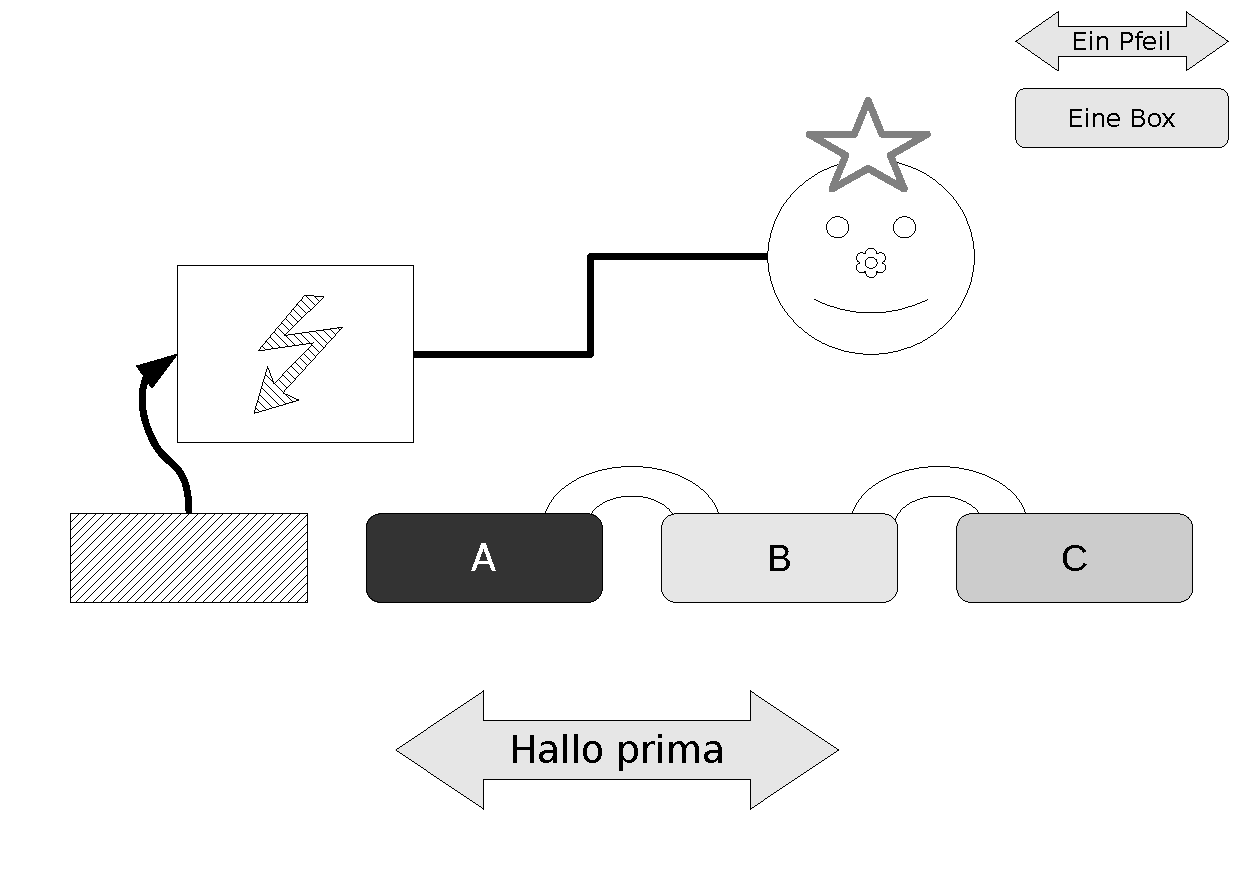
\includegraphics[width=.9\textwidth]{zeichnung.eps}
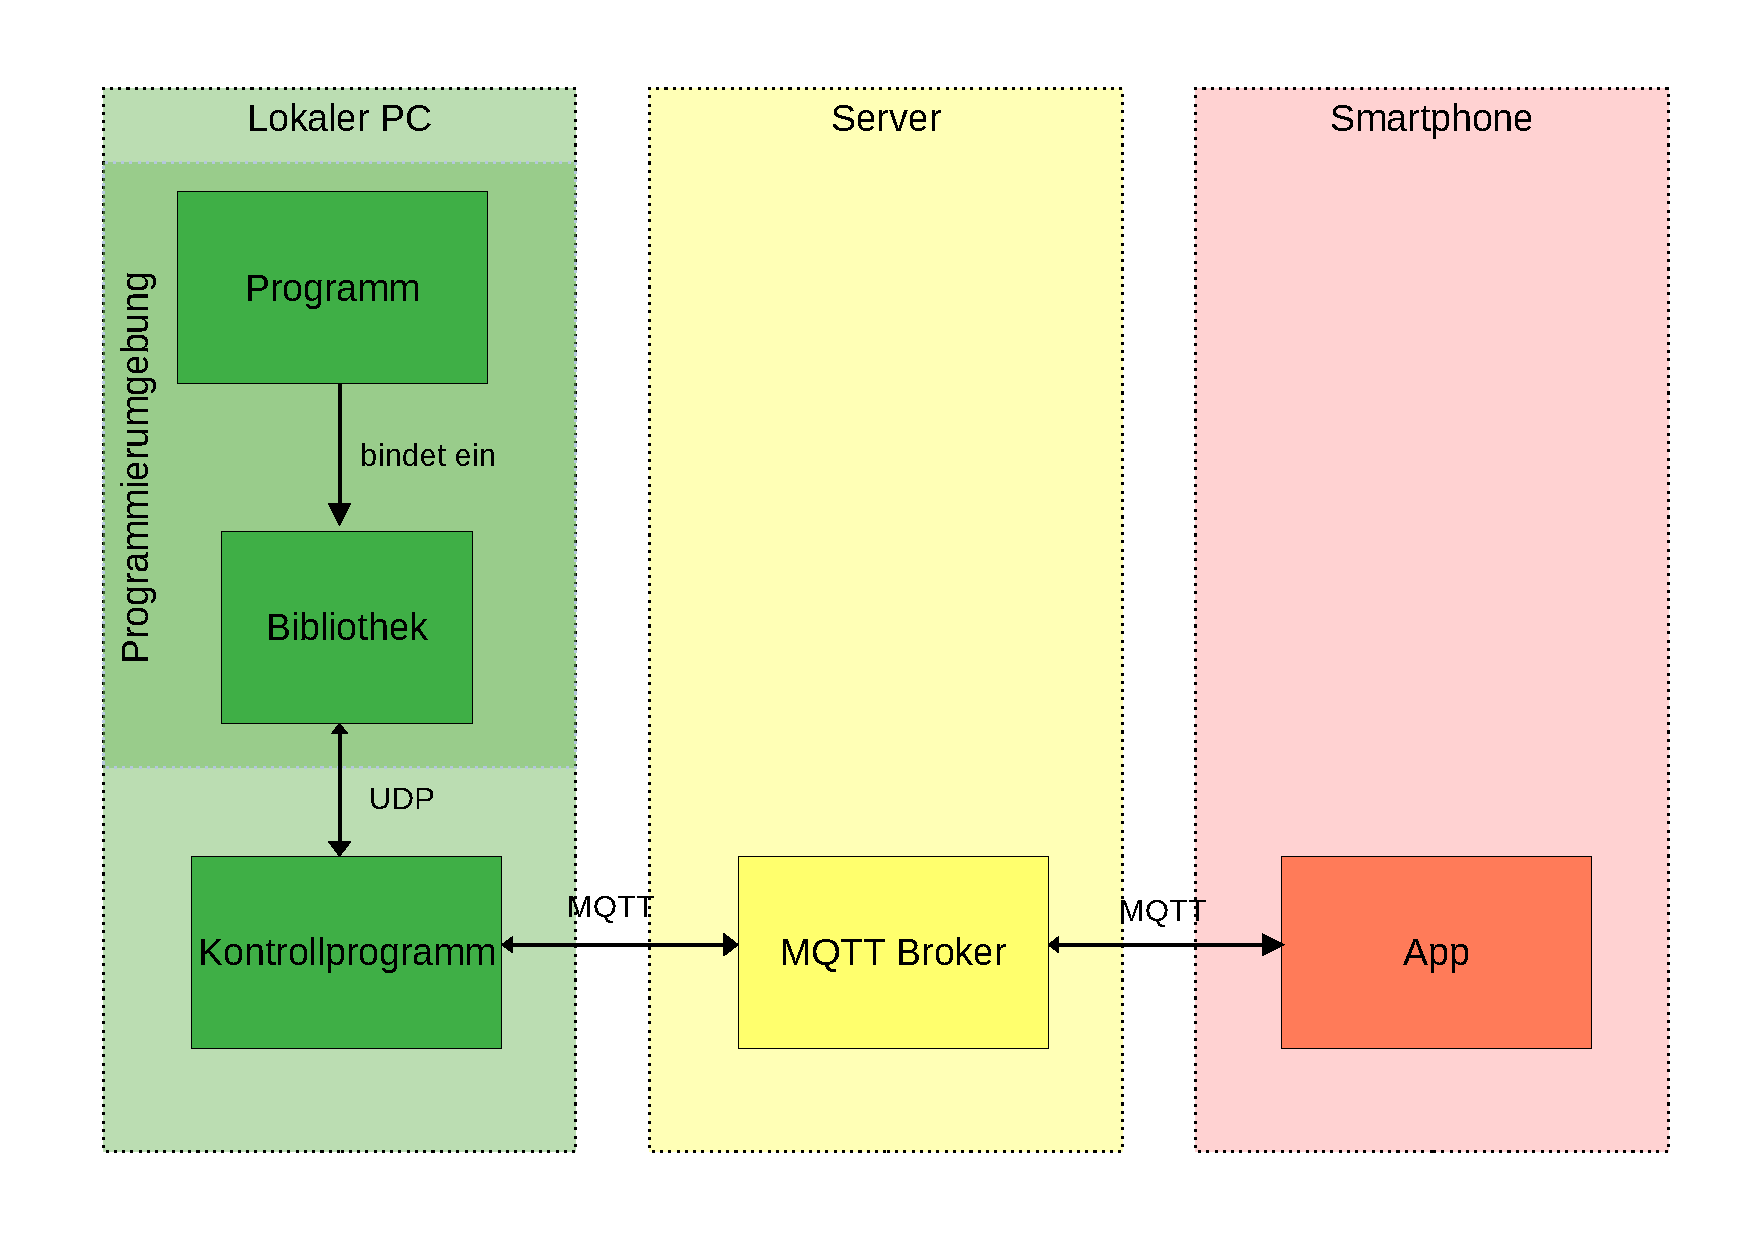
\includegraphics[width=\textwidth]{images/framework.pdf}
\caption{System-Aufbau}
\label{fig:design}
\end{figure}
Das Framework arbeitet in drei Bereichen: Auf dem lokalen PC, auf einem Server und auf dem Smartphone.
Auf dem lokalen PC platziert sind sowohl das Kontrollprogramm, die Bibliothek welche die Aufrufe beinhaltet und das vom Entwickler geschriebene Programm.
Programm und Bibliothek bilden zusammen die Programmierumgebung von der aus der Entwickler die volle Funktionalität des Frameworks nutzen kann, indem er in seinem Programm die Bibliothek einbindet.
Diese bildet ein standardisiertes Interface für Funktionsaufrufe.
Startet ein Entwickler einen Aufruf der Bibliothek, kommuniziert diese ihn per UDP dem Kontrollprogramm.
\\
Das Kontrollprogramm erfüllt drei Aufgaben: Die Beantwortung von Sensoranfragen der Bibliothek, dem Zwischenspeichern von Sensorwerten als Puffer und dem Weiterleiten von Ausgabe-Kommandos auf das Smartphone.
Bibliotheksaufrufe werden also per UDP an das Programm gestellt.
Bei Sensoranfragen nimmt dieses Sie an und liefert ebenfalls über UDP den zuletzt zwischengespeicherten Wert zurück.
Damit dieser auch vorliegt werden von der Smartphone App kontinuierlich, periodisch Sensordaten-Aktualisierungen per MQTT an das Kontrollprogramm gesendet.
Das Kontrollprogramm wiederum sendet Ausgabe-Kommandos per MQTT an die Smartphone-App.
\\
Die Smartphone-Anwendung beginnt zum Start mit der Sensor-Messdatenerhebung welche Sie wie geschildert an die Kontrollanwendung sendet.
Daneben erwartet Sie Ausgabekommandos der Bibliothek, welche Sie bei Eingang ausführt.
\\
Als Vermittlung zwischen Kontrollprogramm und Smartphone-App dient ein MQTT-Broker.
Dieser nimmt Nachrichten beider Kommunikationspartner an und kontrolliert die Zustellung.
\\
Neben der korrekten Funktiosweise der einzelnen Entitäten hat der Austausch von Nachrichten im Framework große Relevanz.
So müssen Inhalt und Aufbau definiert sein, damit die inneren Algorithmen der Komponenten korrekt arbeiten können.
\section{Nachrichtenformate}
Ein einheitliches Kommunikationsformat ist für den Nachrichtenaustausch unabdingbar.
Der ausgearbeitete Standard definiert Nachrichten in einem Klartextformat.
Als Darstellungsform wird JSON verwendet.
\\
Die Nachrichtenformate werden als Vorlagen in einer zentralen Datei abgelegt.
Diese werden in der Bibliothek, dem Kontrollprogramm und in der Smartphone-App abgespeichert und eingelesen.
So ist zentral definiert welche Nachrichten es gibt, welche Felder und Datenformate Sie beeinhalten.
Neben diesen Daten sind zusätzlich noch Bezeichnungen über die nutzbaren Sensoren, sowie den ausführbaren Ausgabe-Kommandos enthalten.
\\
Jede Nachricht weist mindestens die Angabe eines Nachrichtenformat-Typs auf.
Diese sind der Tabelle \ref{tab:message_types} zu entnehmen.
\begin{table}[htbp]
  \centering
  \begin{tabular}{|l|p{30mm}|c|c|}
      \hline
      \textbf{Nachrichtentyp} & \textbf{Quelle} & \textbf{Ziel} & \textbf{Netzwerkprotokoll}\\
      \hline
		sensor\_request & Bibliothek & Kontrollprogramm & UDP\\
       \hline
       sensor\_response & Kontrollprogramm & Bibliothek & UDP\\
       \hline
		update\_request & Smartphone & Kontrollprogramm & MQTT\\
       \hline
		rpc\_request & Bibliothek, Kontrollprogramm & Smartphone & UDP/MQTT\\
       \hline
		rpc\_response & Smartphone, Kontrollprogramm & Bibliothek & UDP/MQTT\\ 
       \hline
  \end{tabular}
  \caption{Nachrichten-Typen}
  \label{tab:message_types}
\end{table}
Die Spalte \textit{Nachrichtentyp} beschreibt die Bezeichnung des Nachrichtentypes.
Zu Übersicht sind noch \textit{Quelle} und \textit{Ziel} der Nachrichten beschrieben.
Außerdem aufgeführt ist das verwendete Netzwerkprotokoll zur Übermittlung.
\\\\
\textit{Sensor\_request}s werden von der Bibliothek an das Kontrollprogramm gesendet.
Ihr Verwendungszweck besteht darin, einen zwischengespeicherten Sensorwert abzufragen.
Daher beeinhaltet Sie neben dem Typ-Bezeichner auch noch das Feld \texttt{sensor\_type}.
Nach Eingang ermittelt das Kontrollprogramm den gewünschten Sensorwert und gibt das Ergebnis zurück.
\\
Eine solche Antwort erfolgt im Nachrichtenformat \textit{sensor\_response}.
Diese beeinhaltet den vom Kontrollprogramm erschlossenen Sensordaten-Wert, \texttt{sensor\_value}, als String.
Sie wird von der Bibliothek entgegengenommen und als float an das aufrufende Programm des Entwicklers zurückgegeben.
Da Aufrufe von der Bibliothek immer blockierend im Call-Response-Schema aufgerufen werden kann es nicht passieren, dass sich responses überholen und die Sensorwerte eines anderen Sensors für den angefragten Sensorwert eingetragen werden.
Deshalb ist die Angabe des gültigen Sensor-Typs für sensor\_responses nicht nötig.
\\
Damit Sensorwerte vorhanden sind muss die Smartphone-App der Kontrollanwendung kontinuierlich gemessene Sensorwerte übermitteln, damit diese in den internen Puffer eingespeichert werden können um bei erhöhten Latenzen Zwischenwerte liefern zu können.
Dies geschieht durch den Nachrichtentyp \textit{update\_request}.
Geltungsgegenstand ist diese Nachricht für alle Art von Sensoren.
Übermittelt wird daher sowohl der Sensor-Typ, als auch der gemessene Sensor-Wert um ihn für die Kontrollanwendung schnell zuordenbar zu machen und Sie in den internen Datenpuffer eintragen zu können.
\\
Der gesamte Ablauf für Sensoranfragen ist in Abbildung \ref{fig:message_flow_requests} zusammengefasst dargestellt.
\begin{figure}[htbp]
\centering
% 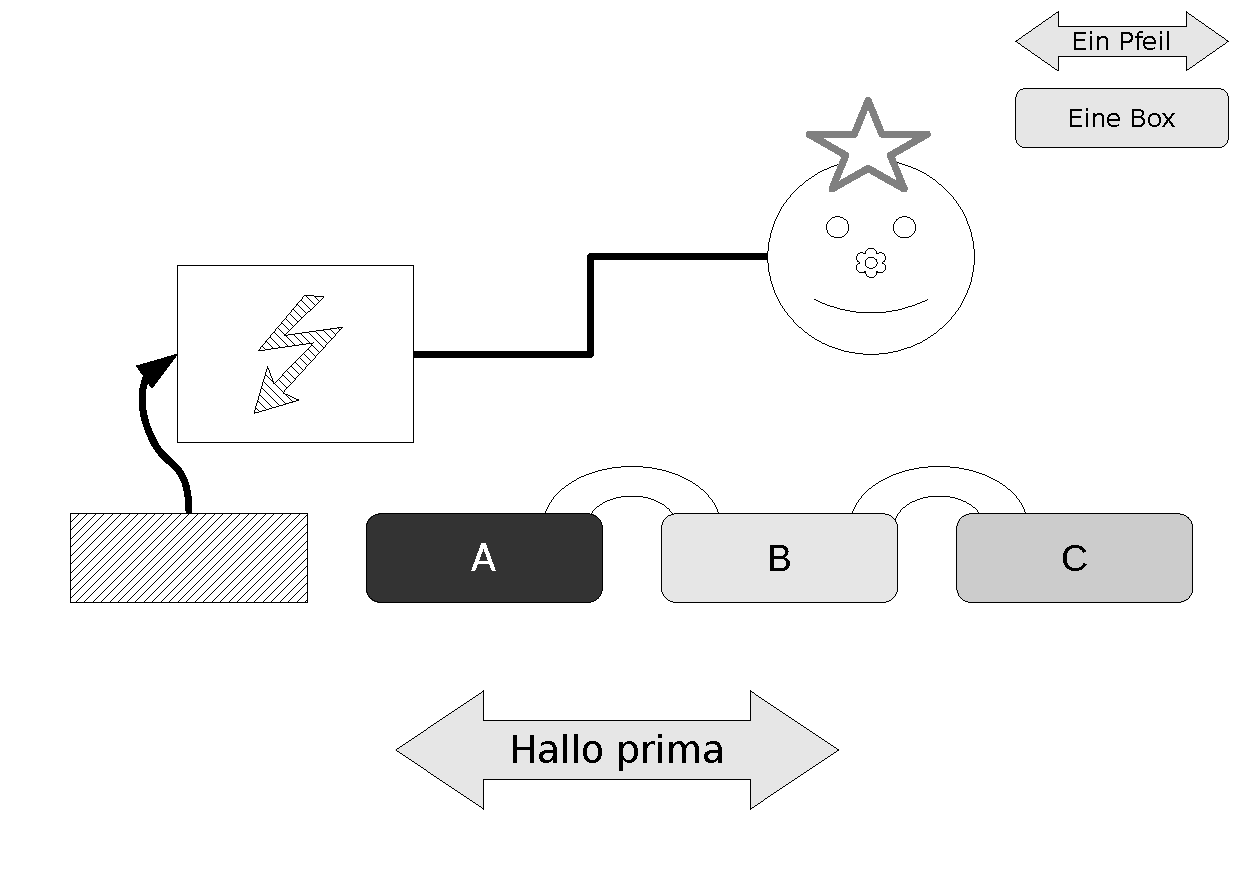
\includegraphics[width=.9\textwidth]{zeichnung.eps}
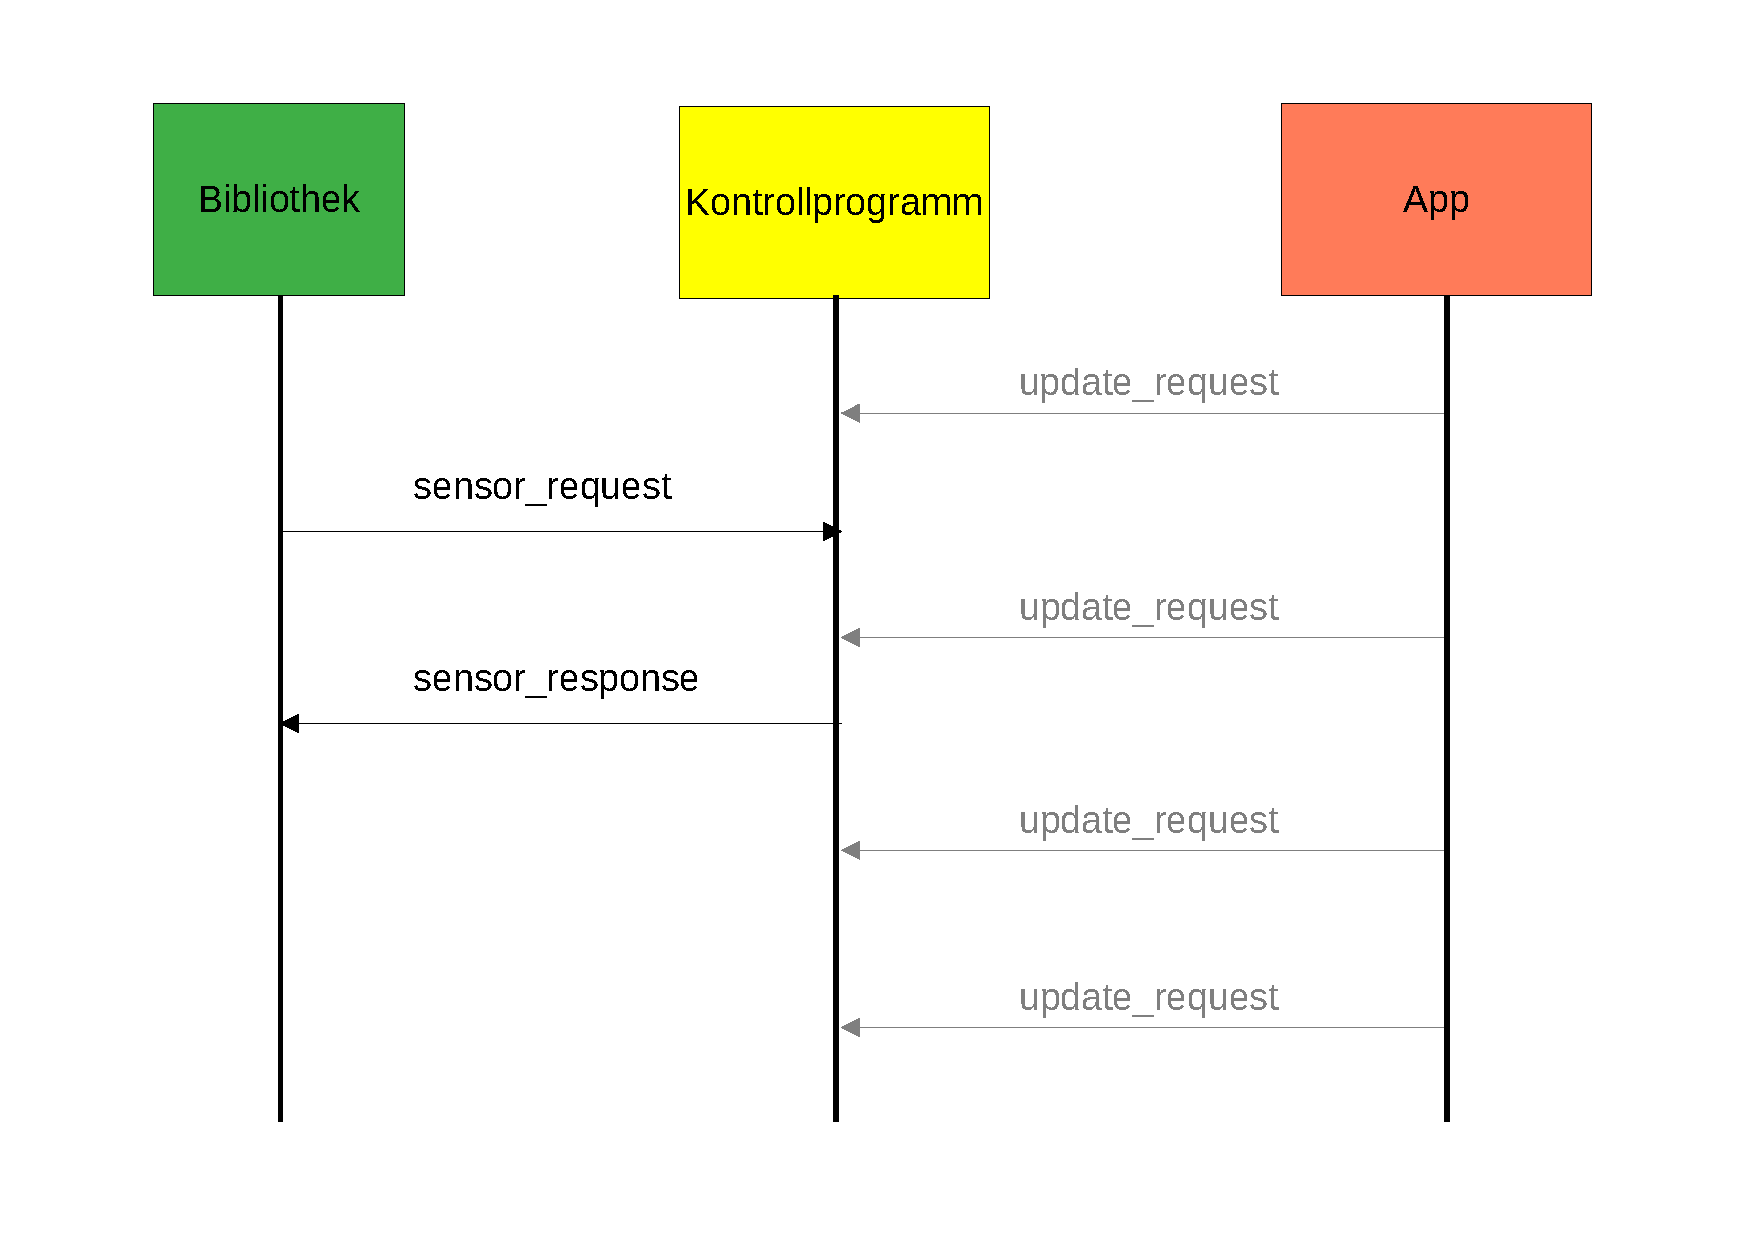
\includegraphics[width=.9\textwidth]{images/message_flow_sensor.pdf}
\caption{Nachrichtenablauf der Sensordatenübermittlung}
\label{fig:message_flow_requests}
\end{figure}
Zu sehen sind die drei Komponenten Bibliothek, Kontrollprogramm und App auf dem Smartphone.
Die Bibliothek sendet sensor\_requests per UDP an das Kontrollprogramm.
Dieses antwortet über UDP mit einer sensor\_response.
Währenddessen sendet die App auf dem Smartphone kontinuierlich update\_requests um neue Messergebnisse der Sensorwerte einzuspeichern.
\\\\
Neben den Sensordaten betreffenden Nachrichten existieren auch Ausgabe-Kommandos um Ausgaben in der Smartphone-App umzusetzen.
Unterscheidbar sind solche Anfragen die lediglich ausgeführt werden sollen und solche , die einen Rückgabewert erwarten.
Für erstere gibt es den Nachreichtentyp \textit{rpc\_request}.
RPC steht für Remote Procedure Call und bezeichnet Funktionsaufrufe die auf einem Client aufgerufen, jedoch auf einem Server ausgeführt werden.
Die Bezeichnung entspricht so nicht dem Konzept, da die die Smartphone-App in diesem Fall die Rolle des Servers einnähme.
Die Voraussetzung einer Client-Server-Anwendung ist nicht gegeben.
Vielmehr tauschen hier gleichwertige Kommunikationspartner Daten aus.
Die Bezeichnung wurde eher unter dem Fokus auf die entfernte Ausführung gewählt.
\\
Der Nachrichtentyp enthält die Felder \texttt{command} und \texttt{value}.
Ersters beeinhaltet eines der spezifizierten Ausgabe-Kommandos.
Das Zweite beschreibt die Größe des Parameters für das Ausgabekommando.
Es ist fast immer befüllt.
Vereinzelt gibt es jedoch auch Kommandos die keinen Parameter benötigen.
Dann bleibt dieses Feld leer.
Die Nachricht wird von der Bibliothek, aufgrund eines Aufrufs des Programmes des Entwicklers erst per UDP an die Kontrollanwendung und von dort aus per MQTT an das Smartphone gesendet.
Die Smartphone-App überprüft bei Eingang den Aufruf und setzt die gewünschte Ausgabe entsprechend um.
\\
Manche Kommandos führen nicht nur Ausgaben aus, sondern erheben zusätzlich noch einen Rückgabewert.
Damit dieser vom Smartphone zurück an die Bibliothek gesendet werden kann gibt es das Nachrichtenformat \textit{rpc\_response}.
Dieses wird erst per MQTT an das Kontrollprogramm und von dort aus per UDP an die Bibliothek gesendet.
Wie bei sensor\_responses können sich die Antworten nicht gegenseitig überholen, was die Übertragung des zugrundeliegenden Ausgabe-Kommandos überflüssig macht.
Nur der ermittelte Wert des Kommandos ist relevant und wird in der Nachricht übermittelt.
\\
Der Nachrichtenablauf wird in Abbildung \ref{fig:message_flow_rpc} nochmal übersichtlich zusammengefasst.
\begin{figure}[htbp]
\centering
% 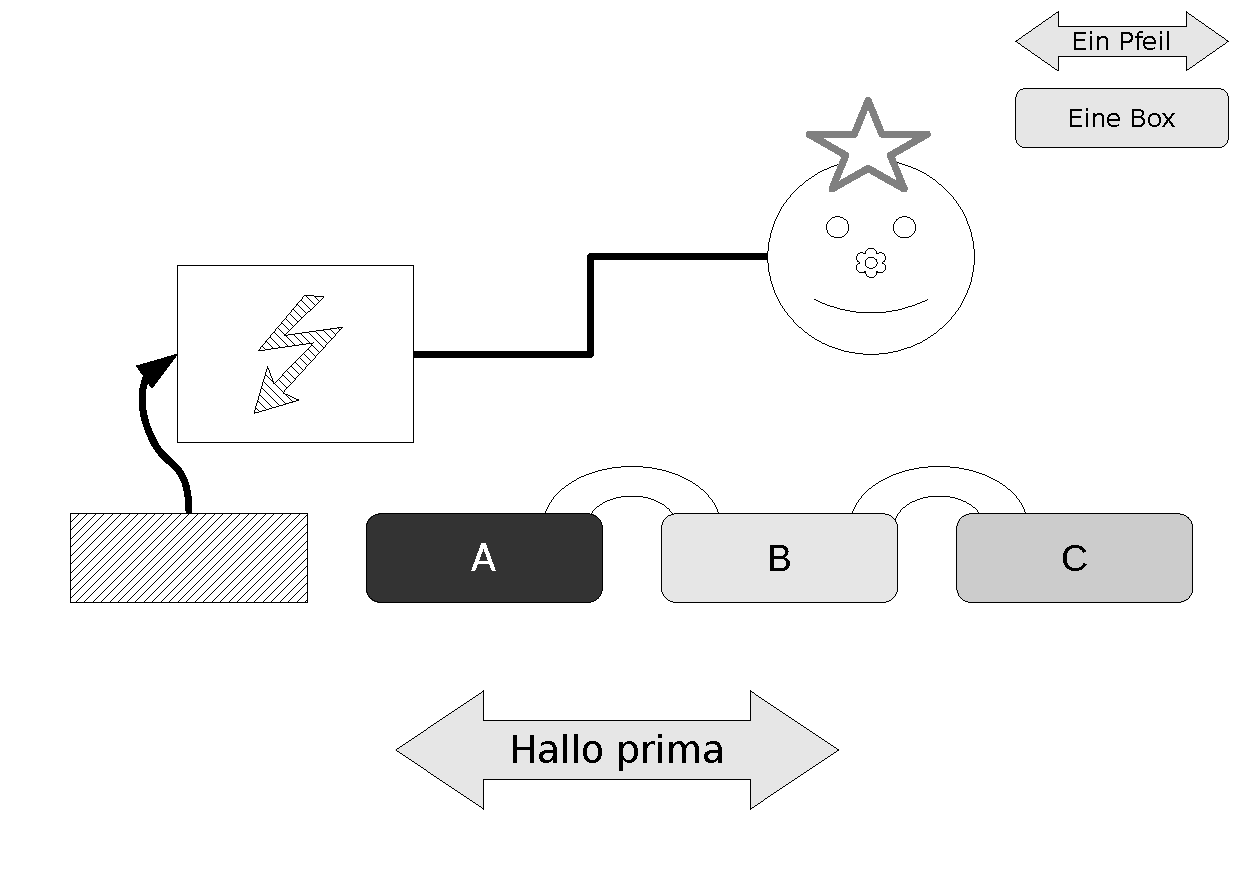
\includegraphics[width=.9\textwidth]{zeichnung.eps}
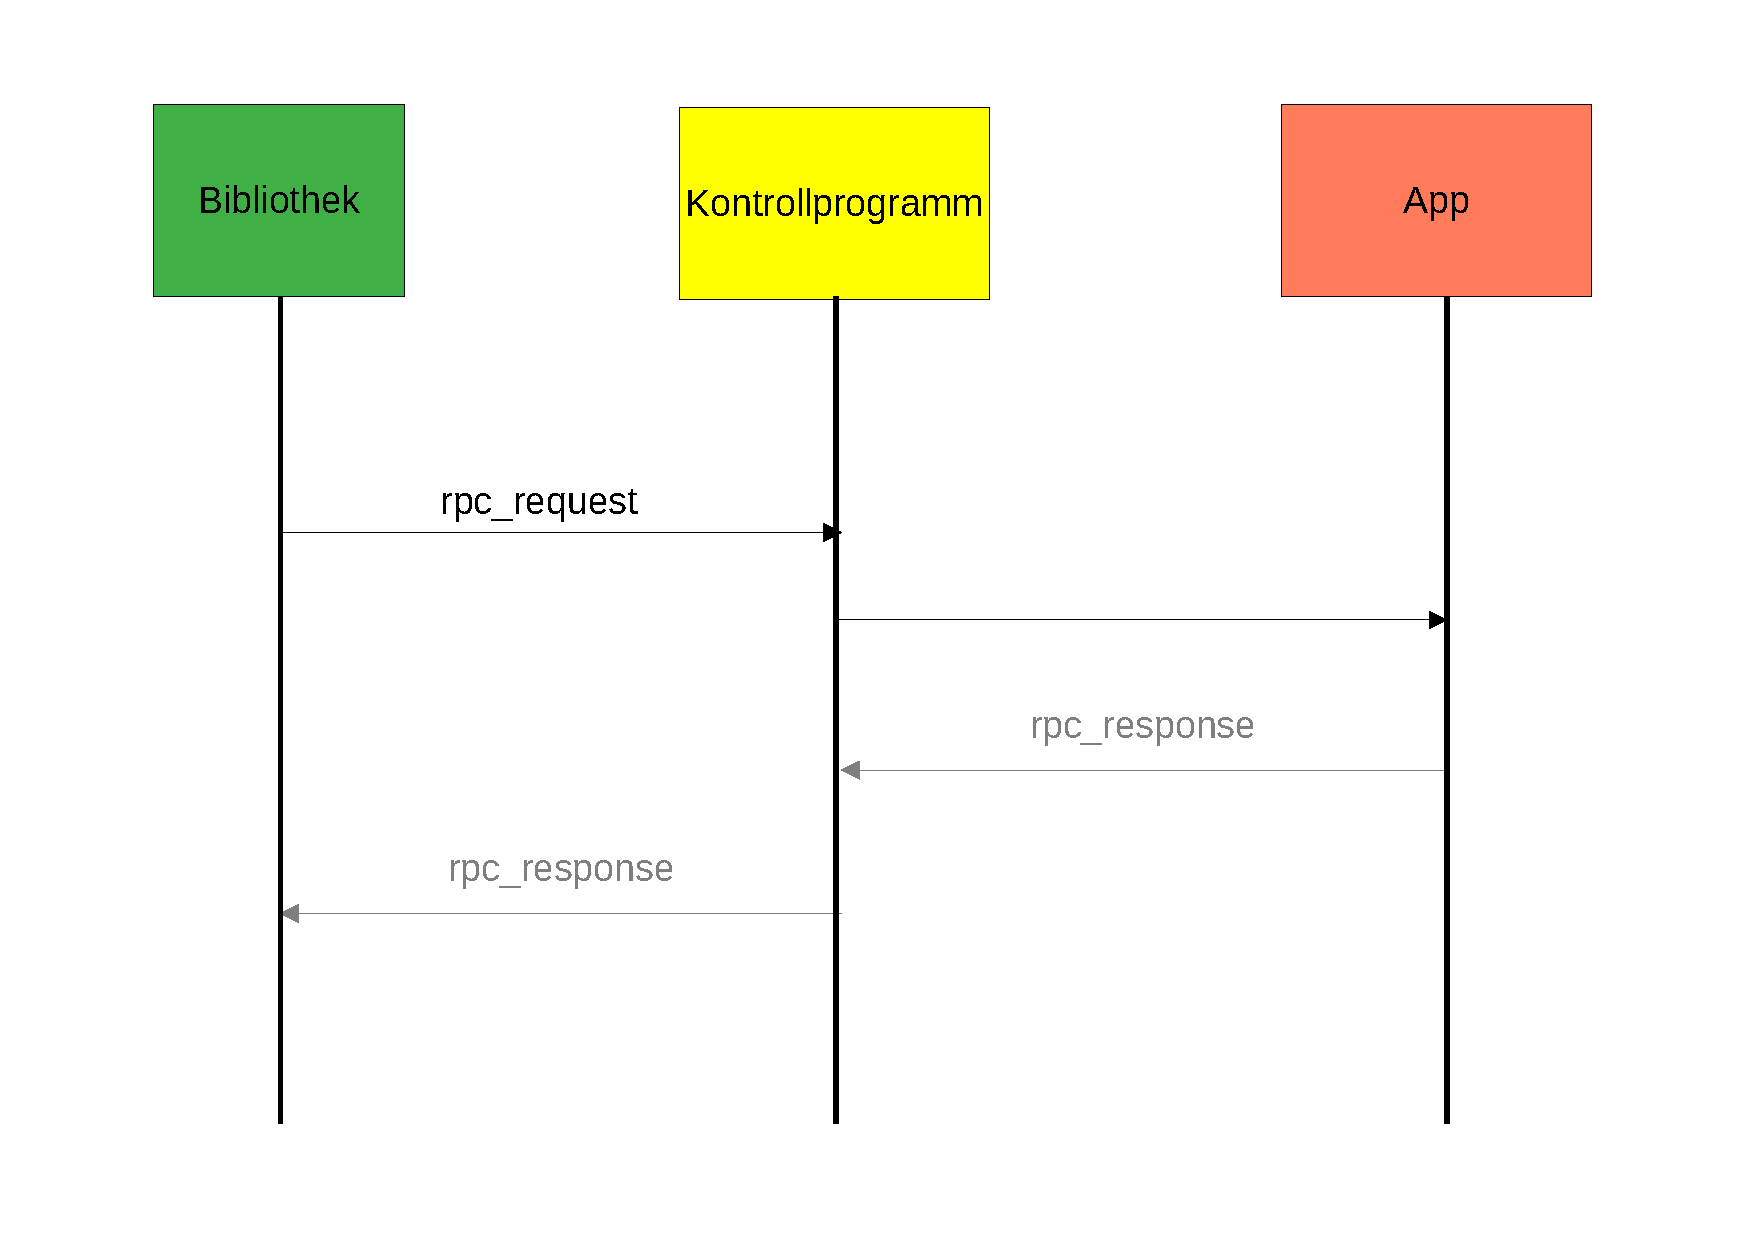
\includegraphics[width=.9\textwidth]{images/message_flow_rpc.pdf}
\caption{Nachrichtenablauf der RPC-Anfragen}
\label{fig:message_flow_rpc}
\end{figure}
Zu sehen sind die drei Komponenten Bibliothek, Kontrollprogramm und App auf dem Smartphone.
Die Bibliothek sendet rpc\_requests per UDP an das Kontrollprogramm.
Dieses leitet die Nachricht per MQTT direkt weiter an die App.
Dort wird das gewünschte Kommando ausgeführt.
Fällt ein Rückgabewert an, wird eine rpc\_response generiert und per MQTT zurück gesendet.
Die Kontrollanwendung leitet die Nachricht dann per UDP weiter an die Bibliothek.
\\\\
Die erstellten Nachrichtenformate decken alle Nutzungszenarien vollständig ab.
Sie bilden ein solides, effizientes Grundgerüst mit Möglichkeit zur Erweiterung.
Diese werden auch vom Serialisierungsformat JSON unterstützt.
Neue Kommandos mit größeren Parameterwerten sind simpel umzusetzen.
Neben Text könnten beispielsweise auch Binärdaten wie Bilder oder Sound-Dateien übertragen werden.
Limitiert werden Sie nur von den darunterliegenden Protokollen UDP und MQTT.

\section{MQTT}
MQTT steht für Message Queuing Telemetry Transport und ist ein Client-Server Protokoll, das auf TCP basiert.
Eingesetzt wird es häufig bei Machine-to-Machine Interaktionen, also Lösungen im IoT-, Smarthome und Automatisierungstechnik-Bereich.
Durch den platzsparenden Header von 2 Bytes und einer maximalen Nachrichtengröße von ca. 260 MB ist es gleichzeitig ein leichtgewichtiges jedoch auch flexibles Protokoll zum Nachrichtenaustausch.
Nachrichten können verschlüsselt übertragen werden.
TLS fungiert dabei auf dem Transportweg als Verschlüsslungsprotokoll.
\\\\
Der Nachrichtenaustausch erfolgt nach dem Observer-Pattern.
Als Publizierungs- und Empfangsplattform dienen hier sogenannte Topics.
Sie funktionieren wie ein Posteingang, dienen allerdings auch der Kategorisierung und Trennung von unterschiedlichen Nachrichten-Kontexten.
Topics können hierarchisch in Topics und Sub-Topics geschichtet werden.
Clients können beim Senden einer Nachricht angeben, auf welchen Topics Sie die Nachricht publizieren möchten.
Clients die die Nachricht empfangen möchten müssen das gewünschte Topic vorab abbonieren.
Neben dem Abbonieren von einzelnen Topics, gegebenenfalls Subtopics, können über Eltern-Topics auch deren Subtopics aggregiert abboniert werden.
\\
Als Vermittlungsstelle dient ein MQTT-Broker.
Dieser bildet die Server-Seite im Client-Server-Konzept.
Senden Clients Nachrichten an ein Topic werden diese vom Broker entgegengenommen und an die abbonierten Clients zugestellt.
Clients können sowohl Sender als auch Empfänger sein.
Das Empfangen der eigenen gesendeten Nachrichten ist möglich.
\\
Alle Clients besitzen darüber hinaus einen Namen, so, dass empfangene Nachrichten auf den Sender zurückgeführt werden können.
Topic-Interne Filter sind ebenfalls möglich, um beispielsweise nur Nachrichten von bestimmten Clients zu empfangen.
\\
Nachrichten können mit einer Quality of Service (QoS), einer Übertragungsgüte, übertragen werden.
Sie gelten sowohl auf dem Weg vom Broker zu einem abbonierendem Client als auch von einem sendenden Client zum Broker.
Topics können also mit einer Güte abboniert und Nachrichten mit einer Güte gesendet werden.
Diese sind in Tabelle \ref{tab:qos} dargestellt.
\begin{table}[htbp]
  \centering
  \begin{tabular}{|c|c|}
      \hline
      \textbf{QOS-Level} & \textbf{Zustellprinzip} \\
      \hline
      0 & At most once \\
		\hline
      1 & At least once \\
      \hline
      2 & Exactly once\\
      \hline
  \end{tabular}
  \caption{Aufgaben}
  \label{tab:qos}
\end{table}
Aufgeführt ist die Übertragungsgüteklasse und das dazugehörige Zustellprinzip.
Letzteres beschreibt die Übertragungsgarantie für Empfänger.
\\
Insgesamt gibt es drei Güteklassen: 0, 1 und 2.
Je höher die QoS-Stufe desto höher die Übertragungsgüte.
Im Gegenzug steigt mit der Übertragungsgüte allerdings auch die Latenz der Übertragung.
\\\\
QoS-Stufe 0 ist die geringste Gütestufe.
Hier werden Nachrichtern einmal übertragen.
Es wird nicht sichergestellt, dass die Nachricht schlussendlich zugestellt wird. 
Der Sender überträgt die Nachricht nur einmal an den Broker und dieser Sie auch nur einmal an den Empfänger.
Es gibt keine Übertragungsbestätigung an keiner Zwischenstation.
Deshalb kann ist die Garantie lediglich dass die Nachricht im besten Falle einmal zugestellt wird.
\\
Bei der QoS Stufe 1 muss zwischen Sender und Empfänger unterschiden werden.
Sender senden die Nachricht immer wieder, bis Sie eine Bestätigung vom Broker bekommen.
Dieser sendet Sie immer wieder an den Empfänger bis dieser den Eingang einmal bestätigt.
Es kann durch die wiederholte Sendung jedoch vorkommen, dass eine Nachricht mehrmals gesendet wird.
Deshalb ist die Garantie hier lediglich \textit{mindestens einmal}, da nicht sichergestellt werden kann ob eine Nachricht mehrmals eingegangen ist.
\\
QoS 2 ist die höchste Gütestufe.
Sender übertragen die Nachricht einmal an den Broker und warten dann auf die Bestätigung, senden also nicht fortwährend die gleiche Nachricht bis Sie einmal bestätigt wird.
Der Broker sendet Sie dann einmal an alle abbonierten Clients und wartet auf die Bestätigung.
Nachteilig ist hier vor allem die hohe Wartezeit sowie das Fehlschlagen einer Übertragung, sollte das Timeout auslaufen.
Dafür kann der einmalige Empfang der Nachricht garantiert bestätigt werden.
\\\\
Wie eingangs erwähnt ist die Übertragungsgüte sowohl von sendenden Clients, als auch von abbonierenden Client individuell einstellbar.
Damit die verlangte Güte sichergestellt werden kann müssen Sender und Empfänger mit der gleichen Güte senden bzw. ein Topic mit der gleichen Güte-Stufe abbonieren.
Wird ein Topic mit einer geringeren Güte abboniert, als die Nachricht versendet wird, wird die Nachricht mit der geringeren Güte des Abbonenten übertragen.
Wenn eine Nachricht mit geringerer Güte auf einem Topic publiziert wird, als Clients das Topic abboniert haben, wird die Übertragung mit der geringeren Güte-Stufe des publizierenden Clients übertragen.
Zusammenfassend gilt: Unterscheiden sich Sender- und Abbonenten-Güteklassen geschieht die Übertragung mit der geringeren Güteklasse.

\chapter{Android Anwendung}\label{chap:app}
Die Android-Anwendung ist eine der drei zentralen Bestandteile des Frameworks.
Sie dient dazu Sensormessprozesse zu starten, Sensordaten zu übermitteln und Ausgabe-Kommandos auszuführen.
Für diese bietet Sie unterschiedliche UI-Elemente in einer Activity, der RootActivity ein.
Sie ist zentrale UI Schnittstelle für sämtliche Formen der Ausgaben.
Diese sind: eine Signal-Led und ein Textfeld.
Neben UI Elementen gibt es zusätzlich noch die haptische Ausgabe der Vibration.
\\
Für die Grundfunktionalität benötigt die Kontrollanwendung des Frameworks Sensordaten welche Anschließend versendet werden müssen.
Versandt werden die Nachrichten über einen Service, der im Hintergrund ausgeführt wird, dem MQTT-Service.
Die Sensordatenerhebung funktioniert über sogenannte SensorEventListener.
Sie starten Sensormessprozesse und überwachen diese auf neue Werte.
In einem solchen Fall senden Sie über den MQTT-Service update\_requests an das Kontrollprogramm.
Die Anwendung versendet neben dieser Nachrichtenart auch noch rpc\_response-Nachrichten.
Erstellt werden diese von der Klasse JsonMessageWrapper.


\section{Funktionsablauf}
Die Erhebung der Messwerte erfolgt zum Start der Anwendung.
Ein Ablaufplan ist in Abbildung \ref{fig:app_flow} zu sehen.
Asynchrone Schritte sind mit einem \textit{A} markiert.
\\\\
\begin{figure}[htbp]
  \centering
  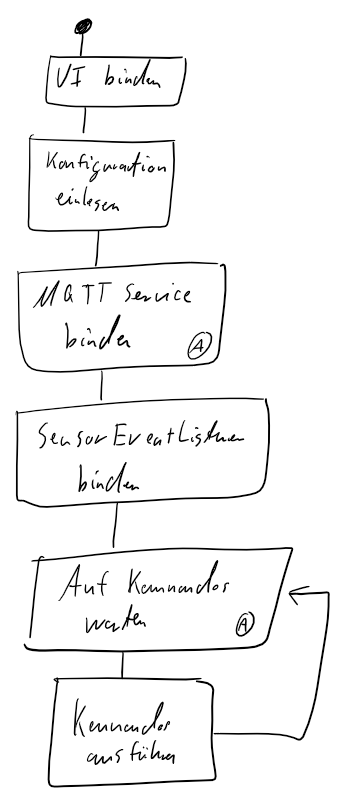
\includegraphics[height=0.8\textheight]{images/app_ablauf.png}
  \caption{Ablaufdiagramm Android Anwendung}
  \label{fig:app_flow}
\end{figure}
In der Root-Activity werden zuerst alle UI-Elemente eingebunden um Sie über Kommandos zu manipulieren.
Anschließend werden Konfigurationsdaten eingelesen.
Insgesamt gibt es zwei Konfigurationsdateien: config.json und protocol.json.
In Ersterem ist zum Beispiel der Hostname des MQTT-Brokers, der Port oder das Topic definiert.
Diese Daten sind für die Übermittlung der Nachrichten per MQTT wichtig.
In protocol.json wird die Form der für das Smartphone relevanten Nachrichtenformate update\_request und rpc\_response definiert.
Außerden sind dort die unterstützten Sensoren und Ausgabekommandos beschrieben.
Relevant werden diese bei der Entscheidungsfindung bei Eingang eines rpc\_requests, wenn determiniert werden muss welche Aktion die Nachricht beeinhaltet.
\\
Nach dem Einlesen der Konfigurationen wird der zur Kommunikation verwendete MQTT Service eingebunden.
Dies geschieht asynchron.
Über eine ServiceConnection wird beim erfolgreichen einbinden über eine Callback-Methode der weitere Verlauf definiert.
Die Root-Activity speichert dann die Referenz auf den Service und der Service die Referenz auf die Root-Activity.
Grund für dieses gegenseitige Einbinden ist, dass Nachrichten im MQTT Service in einem seperaten Thread behandelt werden.
Bei RPC-Requests müssen jedoch UI-Elemente verändert werden können.
Dies ist ohne weiteres nicht aus dem Service heraus möglich.
Mit einer Referenz auf die Activity kann der Service UI-Ändernde Funtionen auf der Activity ausrufen.
Android unterbindet jedoch UI-Manipulationen durch Threads die nicht der UI-Thread sind.
Dieses Problem wird durch die Methode \textit{runOnUiThread} umgangen, welche die Änderung in der Ausführungswarteschlange des UIThreads einreiht.
Der Service baut eine Verbindung zu einem MQTT Server auf.
\\
Beim Einbinden des MQTT Servers stellt dieser eine Verbindung zu einem in config.json definierten MQTT-Broker und Topic her.
\\
Ist der Service final eingebunden können die Sensormessprozesse gestartet werden, da Messdaten nun zuverlässig gesendet werden können.
Verschiedene SensorEventListener werden nun gestartet und zentral in einem SensorEventListenerContainer gesammelt gespeichert und die Messprozesse jeweils angestoßen.
Somit ist die Startroutine der Mobilen Anwendung abgeschlossen.
Auf Nachrichten wird nun nur noch im MQTT-Service in einem MessageListener mit entsprechendem Callback reagiert.
\\\\
Die Funktionsweise der Sensordatenübertragung wird in Abbildung \ref{fig:sensor_event_listener} nocheinmal zusammenfassend dargestellt.
\begin{figure}[htbp]
  \centering
  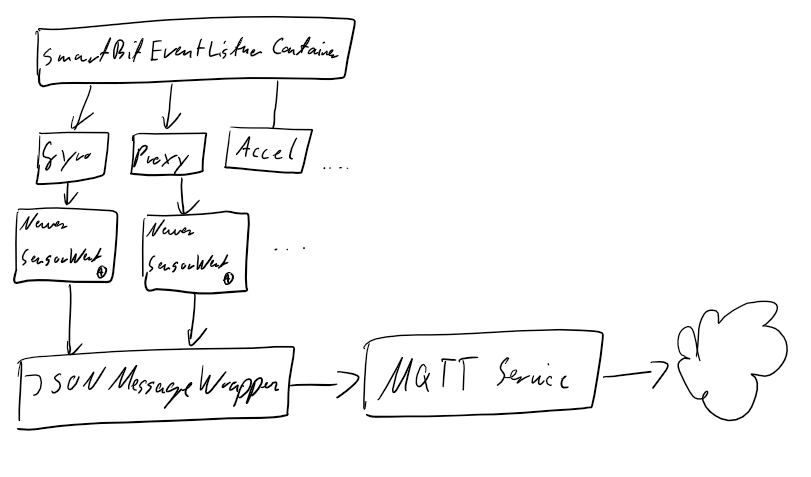
\includegraphics[width=.9\textwidth]{images/sensor_event_listener.png}
  \caption{Ablaufdiagramm SensorEventListener}
  \label{fig:sensor_event_listener}
\end{figure}
Die Klasse \textit{SmartBitEventListenerContainer} beeinhaltet SensorEventListener für alle Arten von untertstützten Sensoren.
Der Container dient lediglich der Datenhaltung.
Aufgabe der SensorEventListener ist es auf Sensorwert-Änderungen zu reagieren und eine entsprechende Callback-Funktion aufzurufen.
In dieser werden dann über statische Methoden der Klasse \textit{JSONMessageWrapper} update\_requests generiert und der gemessene Wert eingesetzt.
Die so generierte Nachricht wird anschließend über den gebundenen MQTT-Service an das vorher definierte Topic versendet.
\\\\
Die Anwendung ist nun betriebsbereit und beginnt bereits erste Nachrichten an die Kontrollanwendung zu senden.
Übermittelt werden die Sensordaten an den Broker mit einer QOS-Stufe von 0.
Verluste von update\_requests sind unproblematisch, da es je nach Taktung sehr schnell neue Sensorwerte gibt die übertragen werden können.
Eine exakte Zustellung ist hier nicht notwendig und verlangsamt eher den Übertragungsprozess.

\section{Sensoren}
Smartphones beeinhalten verschiedene Sensoren die Daten über die Umgebung erfassen können.
In der Android Anwendung werden folgende Sensortypen verwendet:
\begin{itemize}
  \item Lineare Beschleunigungssensoren
  \item Mikrofon
  \item Annäherungssensor
  \item Gyroskop
\end{itemize}

Beschleunigungs- bzw. Lagesensoren messen die Beschleunigung in $m/s^2$ für die drei Bewegungsrichtungen: X-, Y- und Z-Achse in einem festgelegten Zeitraum.
Eine Übersicht über die Anordungen der drei Axen ist in Abbildung \ref{fig:and_axes} zu sehen.
\begin{figure}[htbp]
  \centering
  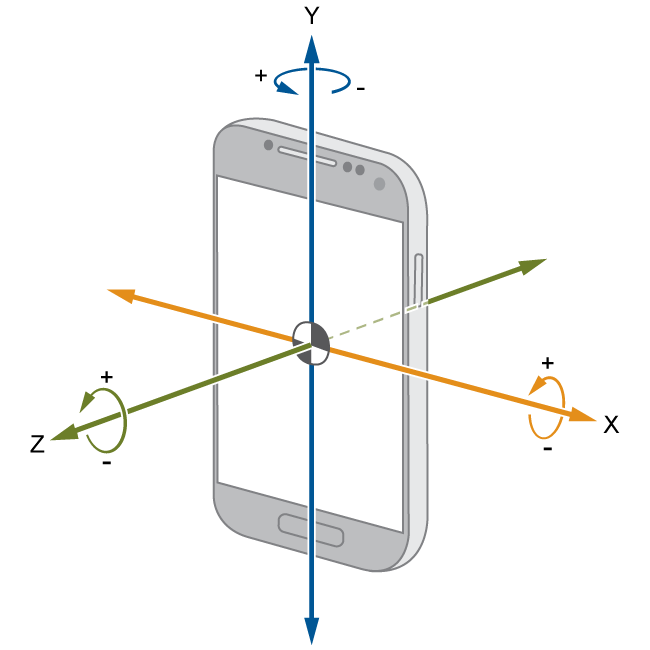
\includegraphics[width=.7\textwidth]{images/android_axes.png}
  \caption{Android-Koordinatensystem}
  \label{fig:and_axes}
\end{figure}
Die X-Achse verläuft horizontal durch das Display des Smartphones hindruch, die Y-Achse vertikal und die Z-Achse durchschneidet das Smartphone in die Tiefe.
\\\\
Die Frequenz mit der Messwerte erstellt werden kann manuell angegeben werden.
Hierfür stehen vier Schnelligkeitsstufen bereit.:
\begin{itemize}
  \item SENSOR\_DELAY\_FASTEST : Kein Verzögerung. Verwendet die Frequenz des Sensors.
  \item SENSOR\_DELAY\_GAME : Verzögerung um 1ms
  \item SENSOR\_DELAY\_UI : Verzögerung um 2ms
  \item SENSOR\_DELAY\_NORMAL : Verzögerung um 3ms
\end{itemize}
Die mit der jeweiligen Frequenz aufgenommenen Beschleunigungssensordaten beeinhalten jedoch auch die Ergbeschleunigung.
Diese muss für die bereinigten, realen Werte zuerst noch von den aufgenommenen Werten subtrahiert werden\cite{accel_g}.
\section{Angaben für die Nachrichtenformate}
Alle Sensordaten besitzen ein festgelegtes Kürzel zur Standardisierung des Nachrichtenverkehrs.
Sie dienen vor allem der Adressierung der jeweiligen Daten in der Middleware und in der Library.
\\
Die Sensortyp Kürzel sind in Tabelle \ref{tab:sensor_types} zu finden. 
\begin{table}[htbp]
  \centering
  \begin{tabular}{|c|c|c}
      \hline
      TYPE-Kürzel & Beschreibung \\
      \hline
      accell\_x & Lagesensor für die X-Richtung \\
      \hline
      accell\_y & Lagesensor für die Y-Richtung \\
      \hline
      accell\_z & Lagesensor für die Z-Richtung \\
      \hline
       gyro\_x & Gyroskopsensor für die X-Richtung \\
      \hline
      gyro\_y & Gyroskopsensor für die Y-Richtung \\
      \hline
      gyro\_z & Gyroskopsensor für die Z-Richtung \\
      \hline
      prox & Näherungssensor \\
      \hline

  \end{tabular}
  \caption{Sensor-Kürzel mit Beschreibung}
  \label{tab:sensor_types}
\end{table}


\section{Kommandos und Ausgaben}
Für die Ausgabe auf dem Smartphone sind verschiedene Kommandos definiert.
Diese sind der Tabelle \ref{tab:command_types} zu entnehmen.
\texttt{CMD-Kürzel} beschreibt die Notation des Kürzels mit dem eine Aktion ausgeführt werden kann.
Diese wird unter \texttt{Beschreibung} kurz zusammengefasst.
\texttt{return} gibt an, ob der Aufruf des Requests eine Antwort rücksendet und somit auch, ob ein Aufruf der Funktion in der Library blockiert oder nur sendet.






\chapter{Kontrollanwendung}\label{chap:server_software}

Für Vermittlung zwischen den Komponenten fungiert eine Server-Anwendung.
Sie ist in Python geschrieben und vermittelt zwischen UDP-Anfragen auf der einen Seite vom Client aus und MQTT-Anfragen vom Smartphone auf der anderen Seite.
User können über die Library RPC-Anfragen oder Sensor-Anfragen an den Server stellen.
Dies geschieht in form von JSON-Anfragen die per UDP übermittelt werden.
Der Server ist unter der localhost-Adresse 127.0.0.1 auf dem Port 5006 erreichbar.
\\
Für die MQTT-Verbindung kommt dabei die unter OpenSource-Liznenz stehende MQTT-Library Paho der Eclipse-Foundation zum Einsatz. \cite{paho}


\section{Anforderungen}
Aus den Anforderungen ergeben sich folgende Aufgaben die der Server umsetzen muss:
\begin{itemize}
\item Sensoranfragen schnell beantworten
\item Anfragen die Funktionen auf dem Smartphone starte, müssen schnell an das Smartphone weitergereicht und gegebenfalls wieder beantwortet werden.
\end{itemize}
Damit Sensoranfragen schnell beantwortet werden können, werden die aktuellen Sensorworte fortlaufend vom Smartphone an den Server übermittelt.
Dieser speichert Sie dann, sobald ein Sensorwert gemessen und übermittelt wurde in eine interne, threadsichere Datenstruktur.
Hierdurch wird insbesondere der Latenzunterschied zwischen Smartphone und Localhost berücksichtigt.
UDP Anfragen per Localhost haben eine wesentlich geringe Latenz als MQTT-Anfragen, auf die das Smartphone reagieren muss.
Durch das Cachen auf dem Server liegen bei Anfragen per UDP, also von der Library aus, immer Sensordaten vor.
\\
Um Funktionsanfragen zeitnah auszuführen müssen unterschiedliche Netzwerklatenzen berücksichtigt werden.
Die Übermittlung erfolgt asynchron zwischen Library und Smartphone, wobei zu erwarten ist dass Übermittlungen an das Smartphone mit einer höheren Latenz übertragen werden, als Anfragen zwischen Library und Server, da sich beide auf dem gleichen Host befinden.
Die Verbindung zwischen Library und Server erfolgt darüber hinaus über localhost und somit über ein Loopback-Device.
Loopback-Devices reichen Netzwerkpakete nicht herkömmlich über ein physisches Netzwerkinterface weiter sondern stellen ein virtuelles Gerät dar, dessen Übertragungsrate an die CPU gekoppelt ist.
Die Bandbreiten sind dadurch sehr hoch und die Latenzen gering.
\\
Um die Latenzen und die damit verbundenen unterschiedlichen Auftrittszeitpunkte von Anfragen zu berücksichten, sowie eine möglichst effiziente Abarbeitung der selbiger zu ermöglichen wird eien paralelle Algorithmusstruktur verwendet.

\section{Interner Aufbau}
Die Serveranwendung mit dem Namen server.py ist aufgeteilt in einen Datenverwaltungsteil, DataHandler, und eine MQTT Anbindung, MQTTHandlerThread.
Da die Sensorwerte des Smartphoens vorrätig gehalten werden, wird außerdem eine Datenklasse für diese, SensorDB, intern gehalten.
Eine Übersicht über die Komponenten ist Abbildung \ref{fig:serverUml} zu entnehmen.
\begin{figure}[htbp]
  \centering
  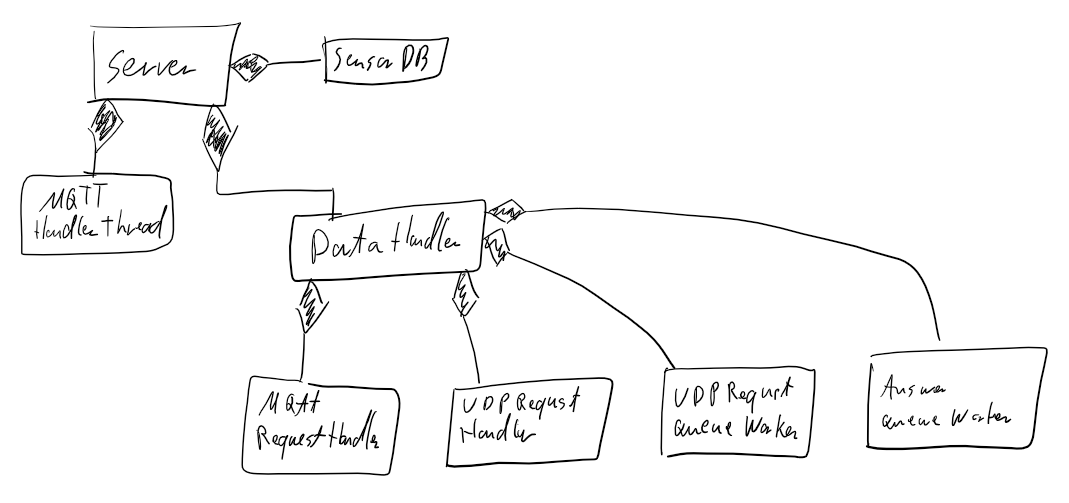
\includegraphics[width=.8\textwidth]{images/ServerUml.png}
  \caption{UML Digaramm Server}
  \label{fig:serverUml}
\end{figure}
\\
DataHandler wiederrum teilt sich nochmal auf in vier seperate Funktionen, die als Threads nebenläufig laufen: MqttRequestHandler, UDPRequestHandler, UDPRequestQueueWorker und AnswerQueueWorker.
\\
Die Funktionsweise und Zwecke dieser Threads wird im Folgenden an zwei Beispielen erläutert.
Für das erste Beispiel wird Abbildung \ref{fig:serverMqttReqPath} betrachtet.
Zu sehen ist ein MQTT-Request, also eine Anfragen des Smartphones, dass über MQTT an den Server gesendet wird.
Schnittstellen zu MQTT sind in der Abbildung grün, Schnittstellen zur Library per UDP, sind blau markiert.
\begin{figure}[htbp]
  \centering
  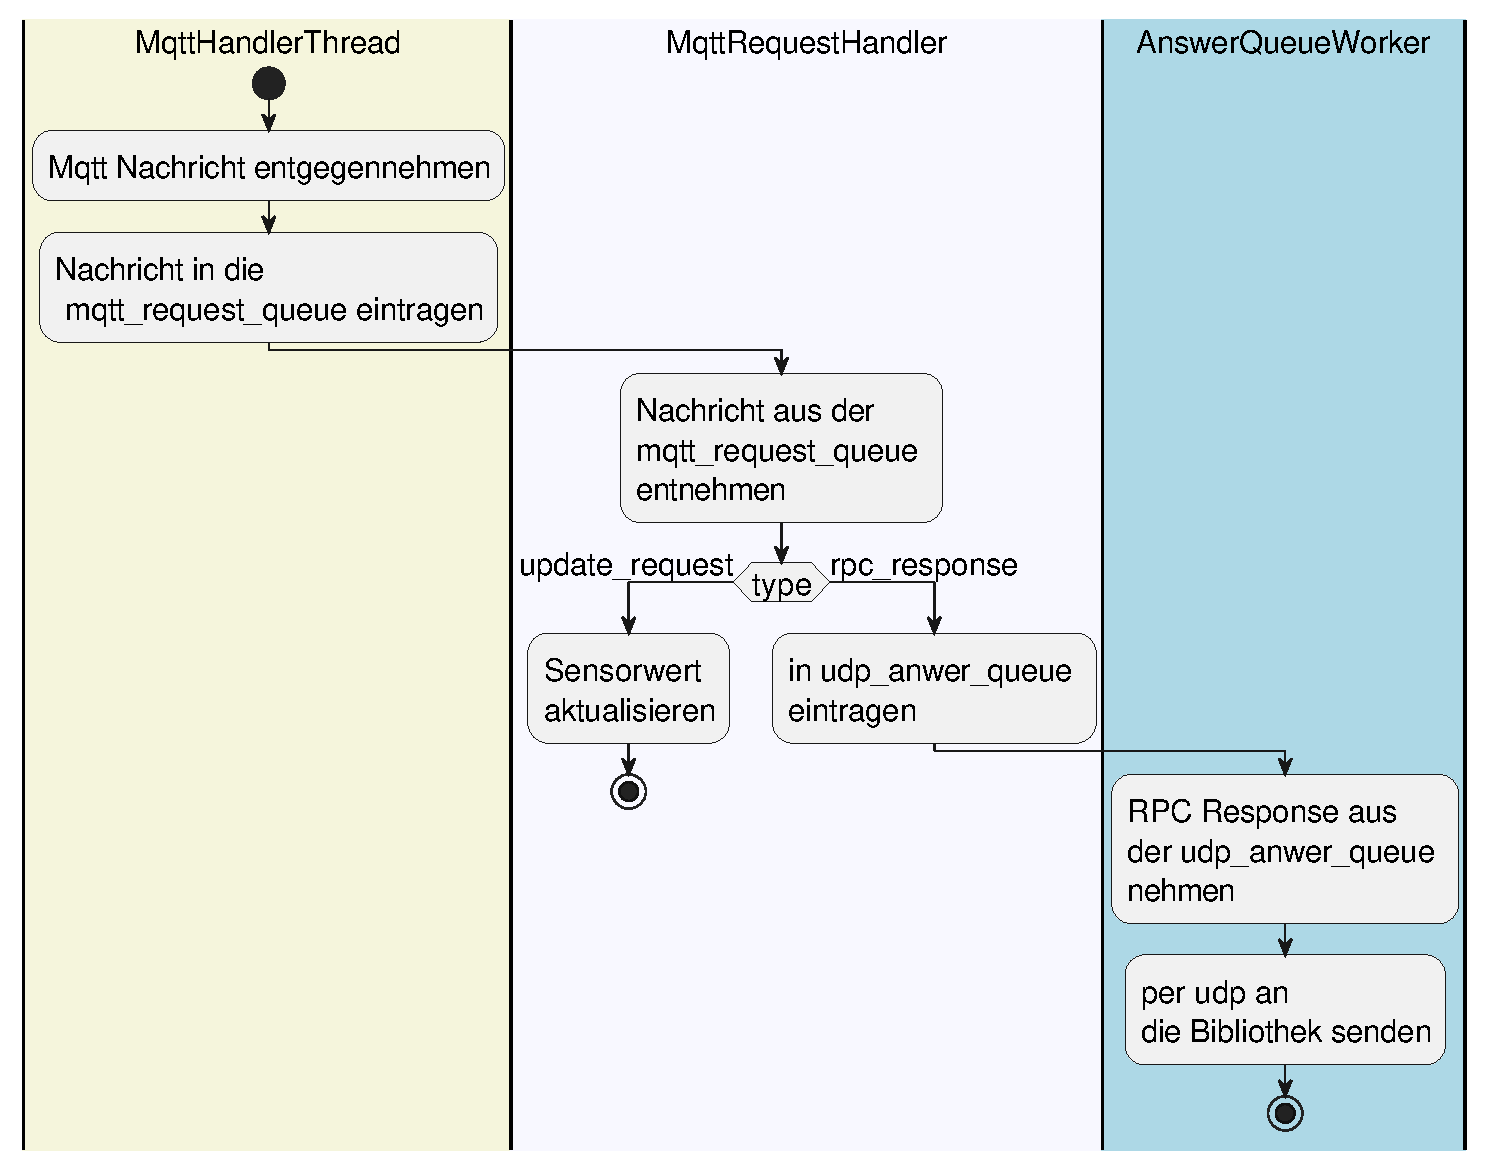
\includegraphics[width=.8\textwidth]{images/MqttRequestServerPath}
  \caption{Ablaufdiagramm MQTT Request}
  \label{fig:serverMqttReqPath}
\end{figure}
\\
Erreicht ein MQTT Request den Server wird es im MQTTHandlerThread entgegengenommen.
Dieser setzt die Nachricht in eine MQTTRequestQueue ein.
Der MQTTRequestHandler des DataHandlers wartet bis ein Eintrag in der Queue vorhanden ist und nimmt gegebenenfalls eine Nachricht.
Daraufhin wird derTyp des Requests bestimmt.
Handelt sich um ein Sensorupdate muss nur der Sensorwert in der Datenbank aktualisiert werden.
Handelt es sich um eine rpc\_response, also um eine Antwort auf eine vorausgegangenes rpc\_request, dass einen Rückgabewert fordert, wird das request in eine udp\_answer\_queue eingefügt.
Der AnswerQueue Worker wartet, ähnlich wie der MQTT Request Handler, bis eine neue Nachricht vorhanden ist die per UDP an den Client gesendet werden soll und sendet diese dann gegebenfalls ab.
\\

Das zweite Beispiel befasst sich mit dem Ablauf eines UDP-Requests, also einer Anfrage die mithilfe der Library gesendet wurde.
Der Ablauf ist in Abbildung \ref{fig:serverUDPReqPath} dargestellt.
Wie auch schon in der letzten Abbildung sind alle Schnittstellen zum Smartphone grün und alle Schnittstellen zur Library blau markiert.
\begin{figure}[htbp]
  \centering
  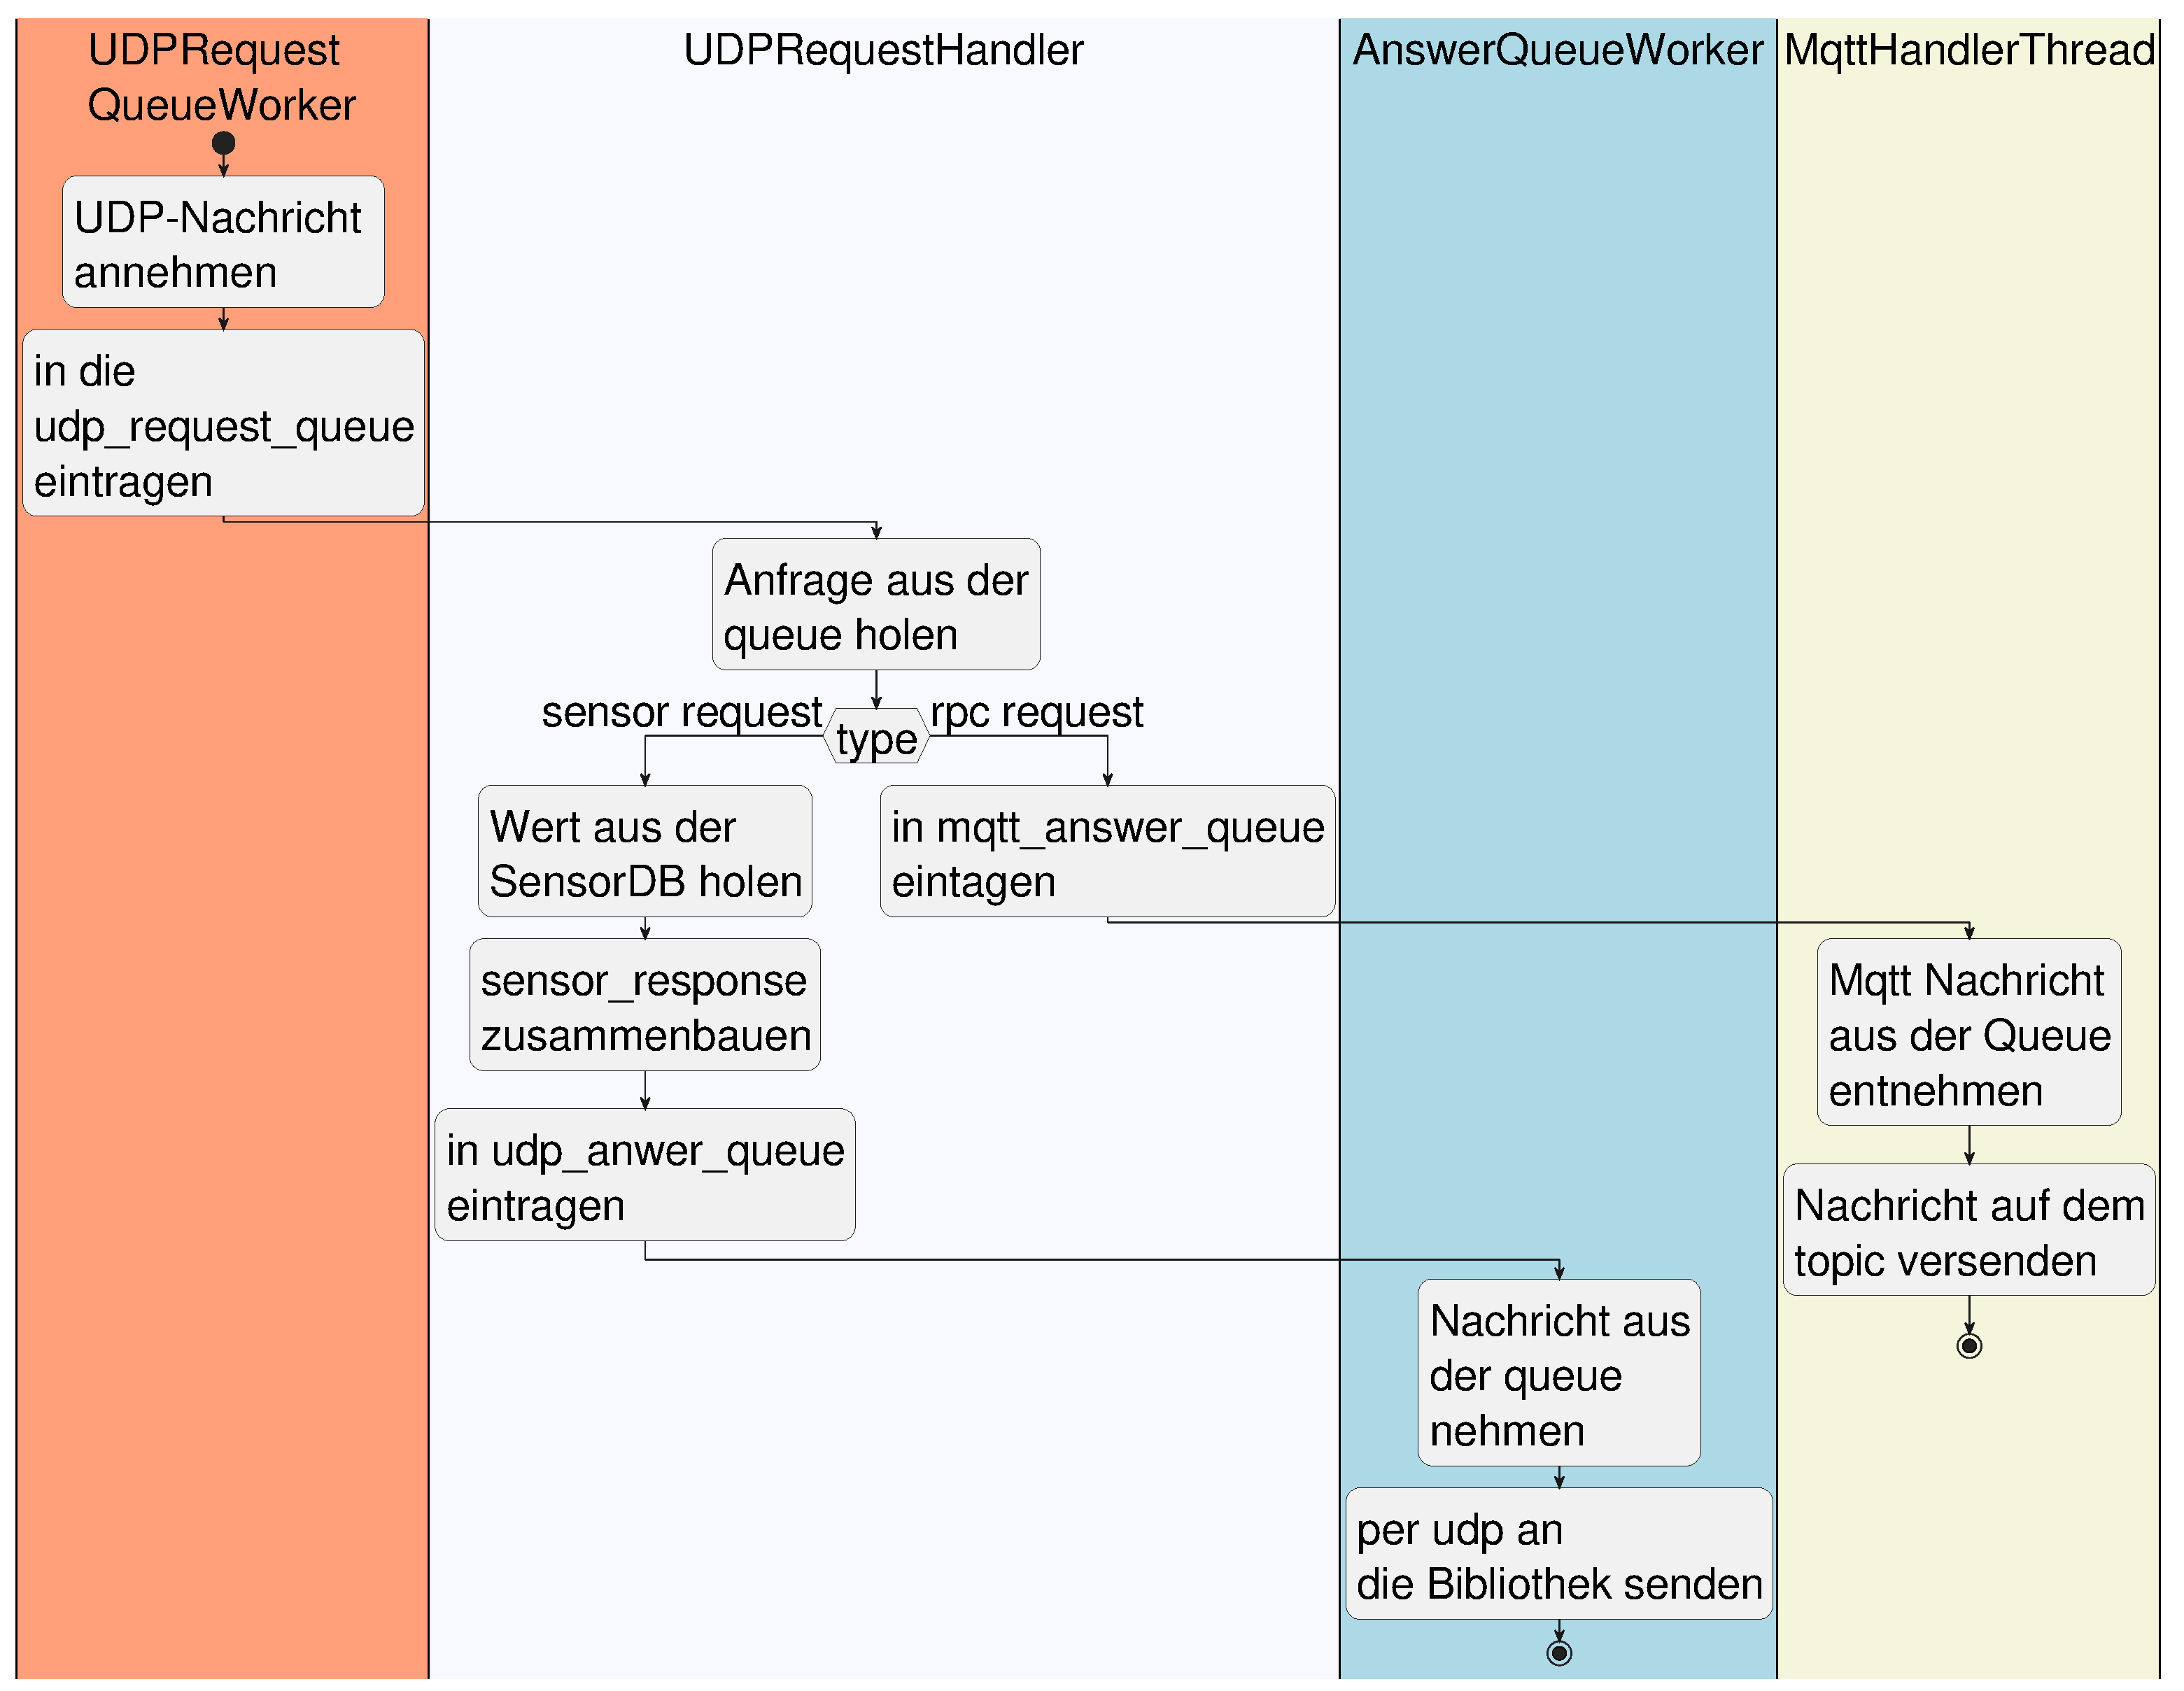
\includegraphics[width=.8\textwidth]{images/UDPRequestServerPath}
  \caption{Ablaufdiagramm UDP Request}
  \label{fig:serverUDPReqPath}
\end{figure}
Erreicht ein UDP Request den Server wird es vom UDPRequestQueue-Worker in eine UDP Request Queue gelegt.
Der UDPRequestHandler-Thread entnimmt die Nachricht und bestimmt den Anfragentyp.
Handelt es sich um eine Anfrage des Types RPC\_Request soll sie Aktionen auf dem Smartphone auslösen.
Sie muss an das Smartphone gesendet werden, was über MQTT möglich ist.
Dafür wird Sie ineine MqttAnswerQueue eingesetzt.
Der MQTTHandlerThread entnimmt Sie und sendet Sie per MQTT ab.
\\
Ist Request hingegen ein SensorRequest, also eine Anfrage auf die ein Sensorwert geantwortet werden soll wird der nachgefragte Sensorwert über die Klasse SensorDB entnommen und in die Udp\_answer\_queue eingetragen.
Der AnswerQueueWorker entnimmt die Anfrage und sendet Sie per udp an die Library zurück.
\\\\
Zusammenfassend erfüllen die Komponenten folgende Aufgaben.
Der MQTTHandlerThread nimmt Nachrichten direkt per MQTT an und gibt die Anfrage weiter.
Außerdem sendet er Nachrichten per MQTT, falls welche anfallen.
\\
Der MQTTRequestHandler kümmert sich um das Verfahren von MQTT Requests.
\\
Der UDPRequestQueue Worker nimmt wie der MQTTHandlerThread Anfragen die per UDP übermittelt wurden an und gibt Sie zur Behandlung entsprechend weiter.
Er sendet jedoch im Gegensatz keine Responses zurück.
\\
Hierfür gibt es den AnswerQueueWorker, dessen einzige Aufgabe es ist Antworten per UDP zurück zu übermitteln.
\\\\
Die Kommunikation zwischen den Threads funktioniert über synchronisierte Queues des queue-Moduls\cite{python_queue} der cpython Implementierung.
Es handelt sich um eine threadsichere Monitorklasse, die einen gleichzeitigen Zugriff zweier unterschiedlicher Threads durch Locks verhindert.

\chapter{Programmierumgebung}\label{chap:libs}
Die Bibliotheken bilden die Einstiegsstelle für Nutzer um die Anwendung fernzusteuern oder Sensorwerte abzufragen.
Funktionsaufrufe liegen jeweils in den Sprachen C, Java und Python vor.
Daten werden wie in Kapitel \ref{chap:architektur} in Abbildung \ref{fig:design} gezeigt per UDP an eine Serveranwendung gesendet.
Diese sendet die Daten dann nach gegebenenfalls per MQTT an das Smartphone weiter, oder wieder per UDP zurück.
\\
Die Bibliotheken senden und empfangen alle jeweils Daten per UDP.
Hierfür werden Sockets benötigt.
Für's Empfangen muss der Socket binded sein.
Die Serveranwendung ist auf dem Port 5006 erreichbar.
Antworten erwarten die Bibliotheken auf dem Port 5005.
\chapter{Evaluation}\label{chap:eval}
\section{Android Anwendung}\label{sec:androidApp}
Für Ausgaben auf dem Smartphone existiert die Android Anwendung Smartbit, die verschiedene Interaktionsmöglichkeiten bereitstellt.
Das Userinterface ist in Abbildung \ref{fig:androidUI} dargestellt..
\begin{figure}[htbp]
  \centering
  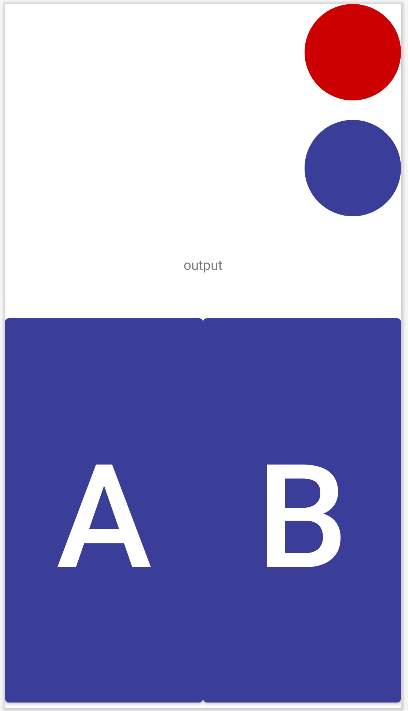
\includegraphics[width=.6\textwidth]{images/android_app_ui}
  \caption{Userinterface Android Anwendung}
  \label{fig:androidUI}
\end{figure}
\\
Die Anwendung besteht aus zwei Leds, einer Signal- und einer Funktions-LED
Ein Textfeld in der Mitte kann zur Ausgabe von Text verwendet werden.
Die beiden Buttons können gedrückt werden.
Neben den sichtbaren Elementen kann die Anwendung das Smartphone außerdem vibrieren lassen.
\\
Die Signal-LED wird für die Ausgabe verwendet.
Aufgabe der Funktions-Led ist die Anzeige eines aktuell ausgeführten Kommandos aufgrund eines rpc\_request.
Leuchtet die LED rot wird gerade ein Vorgang abgearbeitet.
Anschließend verblasst Sie wieder um einen Leerlauf anzuzeigen.
Dieses Designelement wurde zusätzlich implementiert, da gerade sich wiederholende Vorgänge, sowie haptische Vorgänge wie das Vibrieren kein optisches Signal aussenden.
Hält der Anwender das Smartphone beispielsweise nicht in der Hand oder liegt es nicht auf einer harten Oberfläche auf der die Vibration hörbar ist, ist das Vibrieren nicht wahrnehmbar.

\section{Kontrollanwendung}
\blindtext

\section{Programmierumgebung}
\blindtext

\chapter{Fazit}\label{chap:fazit}
\section{Android Anwendung}

\section{Kontrollanwendung}
MQTT QOS 2 zu langsam.
\blindtext

\section{Programmierumgebung}
Nachteil: JSON
\blindtext

\section{Ausblick}
\blindtext

\chapter{Quellen}\label{chap:source}


% Listen wenn überhaupt ans Ende und nicht an den Anfang.
% Meist ist das aber unnötig.
% \listoffigures % Liste der Abbildungen 
% \listoftables % Liste der Tabellen
% \newpage

\bibliographystyle{plain} % Literaturverzeichnis
\begin{btSect}{thesis} % mit bibtopic Quellen trennen
\addcontentsline{toc}{chapter}{Literaturverzeichnis und Online-Quellen}
\section*{Literaturverzeichnis}
\btPrintCited
\end{btSect}
\begin{btSect}{online}
\section*{Online-Quellen}
\btPrintCited
%\bibliography{online}
\end{btSect}
% dann mit "bibtex thesis1" und "bibtex thesis2" arbeiten

\end{document}
;;; Local Variables:
;;; ispell-local-dictionary: "de_DE-neu"
;;; End:


